\documentclass[conference]{IEEEtran}
\IEEEoverridecommandlockouts
\usepackage{cite}
\usepackage{amsmath,amssymb,amsfonts}
\usepackage{algorithmic}
\usepackage{graphicx}
\usepackage{textcomp}
\usepackage{xcolor}
\usepackage{booktabs}
\usepackage{tabularx}
\usepackage{multirow}
\usepackage{url}
\usepackage{hyperref}

\newcolumntype{Y}{>{\centering\arraybackslash}X}

\def\BibTeX{{\rm B\kern-.05em{\sc i\kern-.025em b}\kern-.08em
    T\kern-.1667em\lower.7ex\hbox{E}\kern-.125emX}}

\begin{document}

\title{Cross-Dataset Federated Learning for Floodwater Segmentation: A Literature Review, Proposed Comparative Study, and Experimental Benchmark}

\author{
\IEEEauthorblockN{Taha Ali}
\IEEEauthorblockA{\textit{Department of Computer Science} \\
\textit{FAST-NUCES}\\
Lahore, Pakistan}
\and
\IEEEauthorblockN{M. Usman}
\IEEEauthorblockA{\textit{Department of Computer Science} \\
\textit{FAST-NUCES}\\
Lahore, Pakistan}
\and
\IEEEauthorblockN{Umar Shoaib}
\IEEEauthorblockA{\textit{Department of Computer Science} \\
\textit{FAST-NUCES}\\
Lahore, Pakistan}
}

\maketitle

\begin{abstract}
Accurate floodwater segmentation supports emergency response, exposure assessment, and recovery planning, yet robust models require geographically diverse labeled imagery that is often distributed across separate data owners. Federated learning (FL) permits collaborative model training while raw images remain at their source, but strong cross-dataset heterogeneity can cause unstable optimization and client drift. This review analyzes 20 studies spanning federated optimization, federated semantic segmentation, and remote-sensing flood mapping. It motivates a controlled comparison of FedAvg, FedProx, FedNova, and SCAFFOLD using one independently collected Sentinel-1 flood dataset per client: ETCI 2021, MMFlood, and Kuro Siwo. A common U-Net and harmonized binary target isolate the effect of the FL optimizer. The reviewed evidence shows that advanced algorithms address different types of heterogeneity and that no method is uniformly superior. It also shows that flood studies remain primarily centralized or single-dataset. The resulting gap is the absence of a controlled comparison of established FL optimizers for temporary-floodwater segmentation under real cross-dataset client heterogeneity. In this work, we implement the complete federated learning benchmark across the three silos, evaluating convergence, quantitative segmentation metrics (IoU, Dice/F1, precision, recall, accuracy), cross-dataset fairness, robustness to unequal local computation, qualitative visual error cases, and computational overhead.
\end{abstract}

\begin{IEEEkeywords}
federated learning, floodwater segmentation, non-IID data, Sentinel-1, U-Net, remote sensing, client drift, cross-dataset heterogeneity
\end{IEEEkeywords}

\section{Introduction}
Floods are among the most destructive natural hazards, causing loss of life, displacement, infrastructure damage, and long-term economic disruption. Rapid delineation of inundated areas is therefore important for emergency response, resource allocation, exposure assessment, and post-disaster recovery. Earth-observation systems can survey large or inaccessible areas, while Synthetic Aperture Radar (SAR), particularly Sentinel-1, remains useful during flood events because it operates day and night and is less obstructed by clouds than optical sensing. Flood mapping is nevertheless not identical to general water detection. Permanent rivers, lakes, and reservoirs may already be present before an event; operational mapping must identify temporary inundation without treating all surface water as newly flooded~\cite{bai2021enhancement, bountos2024kuro}.

Semantic segmentation provides a pixel-level solution to this problem. Encoder--decoder networks such as U-Net learn both contextual and spatial information and have produced useful flood masks from Sentinel-1 imagery~\cite{paul2021flood, pechmay2024segmentation}. Their reliability, however, depends on representative annotations across events, climates, land covers, and acquisition conditions. Public flood datasets differ in geographic coverage, sensor preprocessing, label generation, class balance, temporal context, and sample count~\cite{montello2022mmflood, bountos2024kuro, fawakherji2025deepflood}. A model trained on one source can consequently perform poorly when deployed on another domain; recent cross-benchmark evidence confirms that individual-dataset models frequently lose accuracy outside their training distribution~\cite{portalesjulia2025understanding}.

Centralized multi-dataset training can increase diversity, but it assumes that every institution can transfer imagery and annotations to one location. Storage, bandwidth, ownership, governance, and geospatial-security constraints may make that assumption impractical. FL instead sends a shared model to data-holding clients, performs local optimization, and aggregates model updates at a server. Raw imagery remains local, although FL alone is not a formal privacy guarantee because protection against information leakage requires mechanisms such as secure aggregation or differential privacy.

The standard FedAvg algorithm aggregates client parameters in proportion to local sample counts~\cite{mcmahan2017communication}. Its simplicity and communication efficiency make it the principal baseline, but several independent flood datasets create more than an artificial label imbalance. Each client may have a distinct feature distribution, geography, annotation process, class ratio, and dataset size. Local updates can therefore move in conflicting directions. FedProx constrains local deviation from the global model~\cite{li2020federated}; SCAFFOLD uses control variates to correct client drift~\cite{karimireddy2020scaffold}; and FedNova normalizes updates when clients perform unequal amounts of local computation~\cite{wang2020tackling}. NIID-Bench demonstrates that their rankings change across heterogeneity settings, so superiority cannot be assumed without task-specific evaluation~\cite{li2022federated}.

The base study by Islam applied a U-Net and FedAvg to 290 grayscale aerial flood images divided among three simulated clients~\cite{islam2025robust}. Its federated model achieved 0.7186 IoU and 0.8363 F1, compared with 0.7450 IoU and 0.8539 F1 under centralized training; federated recall was higher (0.8883 versus 0.8638) but precision was lower (0.7900 versus 0.8443). These results establish feasibility, yet all clients were partitions of one Kaggle dataset. Their non-IID behavior came from unequal sample counts and flood-pixel ratios, not independent geographic domains. The study also compared only FedAvg and did not report a separate numerical cross-dataset evaluation.

This project addresses that limitation by assigning ETCI 2021, MMFlood, and Kuro Siwo to three independent clients using Sentinel-1 VV/VH inputs and a binary source-annotated flood target. Temporary inundation is the intended application, but annotations do not consistently distinguish it from permanent water across the three datasets. A common U-Net, preprocessing policy, initialization, and training budget isolate the FL optimizer. FedAvg, FedProx, FedNova, and SCAFFOLD are compared under genuine cross-dataset heterogeneity. The objectives are to:
\begin{enumerate}
    \item construct compatible client pipelines while preserving the separation of the three datasets;
    \item compare the four algorithms using IoU, Dice/F1, precision, recall, convergence, and per-client performance;
    \item benchmark federated models against centralized and local-only reference models;
    \item examine whether global gains are distributed fairly across clients rather than dominated by the largest dataset; and
    \item identify the optimization strategy most robust to real flood-domain heterogeneity.
\end{enumerate}

Section~II reviews federated optimization, segmentation under domain shift, and flood models and datasets, then develops the research gap, problem statement, and questions. Section~III presents the proposed methodology and experimental setup for the controlled comparison. Section~IV presents the comprehensive experiments and results, answering all research questions.

\section{Literature Review}
This narrative review covers 20 studies selected for direct relevance to at least one of three components: heterogeneity-aware FL optimization, federated semantic segmentation, or flood segmentation and dataset generalization. Sixteen were published between 2021 and 2025. Four older works are retained because they introduce the four algorithms being compared. Tables~\ref{tab:lit_opt}--\ref{tab:lit_data} report each study's method, dataset, evaluation measures, representative performance, and principal limitation. Scores are reproduced as reported and are not directly rankable because tasks, splits, architectures, and label definitions differ.

\subsection{Federated Optimization Under Heterogeneity}
FedAvg established iterative local training followed by weighted parameter averaging~\cite{mcmahan2017communication}. Its communication savings are substantial, but additional local epochs can amplify drift when client objectives differ. FedProx adds a proximal penalty around the current global parameters and is therefore relevant when independent flood clients produce divergent updates~\cite{li2020federated}. Its behavior depends on the coefficient $\mu$: weak regularization resembles FedAvg, while excessive regularization suppresses useful local learning.

SCAFFOLD estimates server and client control variates to correct local directions~\cite{karimireddy2020scaffold}. Its strong results under severe label heterogeneity make it theoretically attractive for cross-dataset clients, although maintaining control states increases implementation and communication cost. FedNova addresses objective inconsistency by normalizing updates for unequal local work~\cite{wang2020tackling}. Consequently, its central advantage is not fully tested if all clients always execute identical local steps. A sound comparison should use equal computation for the main statistical-heterogeneity experiment and add an unequal-local-step stress test.

NIID-Bench is especially important because it compares all four methods across several non-IID constructions and finds no universal winner~\cite{li2022federated}. However, these are mostly artificial partitions of classification datasets. Islam's flood experiment is closer to the target application, but its clients still originate from one aerial dataset~\cite{islam2025robust}. Table~\ref{tab:lit_opt} shows that optimization evidence is strong, whereas direct evidence for independent flood domains remains absent.

\begin{table*}[t]
\centering
\caption{Literature Survey, Part I: Federated Optimization and the Base Flood-FL Study.}
\label{tab:lit_opt}
\small
\begin{tabularx}{\textwidth}{p{1.8cm}p{0.8cm}p{3.2cm}p{2.8cm}p{2.2cm}p{3.2cm}X}
\toprule
\textbf{Ref.} & \textbf{Year} & \textbf{Method} & \textbf{Dataset(s)} & \textbf{Metrics} & \textbf{Reported Performance} & \textbf{Key Limitation} \\
\midrule
Islam~\cite{islam2025robust} & 2025 & U-Net with three-client FedAvg; centralized comparison & Kaggle Flood Area Segmentation; 116/54/62 client samples & Precision, Recall, F1, IoU, MPA, FWIoU & Centralized/FedAvg IoU: 0.7450/0.7186; F1: 0.8539/0.8363; Recall: 0.8638/0.8883 & Artificial partitions of one aerial dataset; only FedAvg; no separate numeric cross-domain test \\
McMahan et al.~\cite{mcmahan2017communication} & 2017 & Weighted averaging after local SGD & MNIST, CIFAR-10, Shakespeare & Accuracy, Rounds & MNIST target reached in 18 IID rounds vs 626 FedSGD; 173 vs 483 non-IID & Classification/language focus; susceptible to drift under strong domain shift \\
Li et al.~\cite{li2020federated} & 2020 & Proximal local objective around global weights & Synthetic, MNIST, FEMNIST, Shakespeare, Sent140 & Accuracy, Convergence & $\sim$22 percentage-point mean accuracy gain over FedAvg in high straggler setting & Requires tuning $\mu$; no dense segmentation evaluation \\
Karimireddy et al.~\cite{karimireddy2020scaffold} & 2020 & Server/client control variates correct update directions & EMNIST and synthetic tasks & Accuracy, Rounds & Severe EMNIST setting: target in 77 rounds vs 258 for FedAvg; 0.801 vs 0.787 at 1000 rounds & Extra state and communication; classification rather than segmentation \\
Wang et al.~\cite{wang2020tackling} & 2020 & Normalized aggregation for unequal local computation & Non-IID CIFAR-10, VGG-11 & Accuracy & Random local epochs: 73.22\% vs 64.22\% FedAvg; with momentum 77.07\% vs 70.44\% & Main benefit depends on variation in local work; no segmentation task \\
Li et al.~\cite{li2022federated} & 2022 & NIID-Bench comparison across six non-IID constructions & Nine classification/tabular datasets & Accuracy, Convergence & One CIFAR-10 setting: SCAFFOLD 69.8\%, FedAvg 68.2\%, FedProx 67.9\%, FedNova 66.8\% & Artificial partitions and non-segmentation tasks \\
\bottomrule
\end{tabularx}
\end{table*}

\begin{table*}[t]
\centering
\caption{Literature Survey, Part II: Federated Semantic Segmentation and Domain Generalization.}
\label{tab:lit_seg}
\small
\begin{tabularx}{\textwidth}{p{1.8cm}p{0.8cm}p{3.2cm}p{2.8cm}p{2.2cm}p{3.2cm}X}
\toprule
\textbf{Ref.} & \textbf{Year} & \textbf{Method} & \textbf{Dataset(s)} & \textbf{Metrics} & \textbf{Reported Performance} & \textbf{Key Limitation} \\
\midrule
Liu et al.~\cite{liu2021feddg} & 2021 & Episodic learning in continuous frequency space & Multi-centre fundus and prostate MRI & Dice, Hausdorff distance & Fundus Dice: 87.03\% vs 85.01\% FedAvg; HD: 13.07 vs 15.93 & Medical domains; frequency/style assumptions may not represent SAR variation \\
Fantauzzo et al.~\cite{fantauzzo2022feddrive} & 2022 & FL benchmark with local normalization and style transfer & Cityscapes, IDDA & mIoU & Heterogeneous Cityscapes: FedAvg 43.33\%; SiloBN+LAB 53.37\%; rainy unseen 53.99\% & RGB driving scenes; different client scale and appearance physics \\
Miao et al.~\cite{miao2023fedseg} & 2023 & Background-aware loss plus pixel contrastive learning & Cityscapes, CamVID, Pascal VOC, ADE20K & mIoU, Pixel Accuracy & Strong non-IID Cityscapes mIoU: 50.24\% vs 10.40\% FedAvg; CamVID: 63.50\% vs 19.06\% & Artificial class heterogeneity; changes loss and representation mechanism \\
Ma et al.~\cite{ma2024fedst} & 2024 & Diffusion style transfer for cross-client image synthesis & Material, CHAOS medical, race and age segmentation & Dice, VI, MPA & Medical Dice: 0.9233 vs 0.3622 FedAvg; material Dice: 0.8145 vs 0.6754 & High generation cost and additional information-sharing assumptions \\
Tan et al.~\cite{tan2024bridging} & 2024 & Global insight, essential features, and local-global balance & FedFBP, FedCASID, FedInria & mIoU, IoU & FedFBP: 66.70\% vs 63.13\% FedAvg; FedCASID: 74.34\% vs 71.18\% & Remote sensing preprint; land-cover/building tasks; several coupled modules \\
Yu et al.~\cite{yu2025fedsaas} & 2025 & Global class prototypes and local adversarial harmonization & Driving-scene client domains & Accuracy, mIoU & Severe shift mIoU: 48.67\% vs 37.19\% FedAvg; unseen domain: 45.96\% & Exemplar upload and high overhead; RGB driving rather than SAR \\
\bottomrule
\end{tabularx}
\end{table*}

\subsection{Federated Segmentation and Domain Shift}
Federated semantic segmentation adds pixel imbalance and spatial consistency to the optimization problem. FedDG uses episodic learning and frequency-space interpolation to transfer distributional information among medical clients and improve unseen-domain performance~\cite{liu2021feddg}. FedDrive studies autonomous-driving segmentation under statistical and appearance heterogeneity; its results show that naive FedAvg can degrade sharply and that local normalization and style augmentation can recover performance~\cite{fantauzzo2022feddrive}. These studies support evaluation on independent domains, but medical and RGB driving styles differ physically from SAR backscatter.

FedSeg addresses class-heterogeneous segmentation through a background-aware loss and pixel-level contrastive learning~\cite{miao2023fedseg}. FedST uses diffusion-based style transfer to synthesize cross-domain appearances~\cite{ma2024fedst}. Their gains demonstrate that segmentation-specific interventions can exceed optimizer-only baselines, but they alter losses, representations, or data distributions. They are therefore related work rather than fair replacements for the proposed controlled optimizer comparison.

GeoFed is the closest remote-sensing precedent. It models coupled class-distribution and object-appearance heterogeneity across institutions and improves land-cover/building segmentation over FedAvg~\cite{tan2024bridging}. FedSaaS similarly aligns local and global class representations with prototypes, contrastive losses, and adversarial harmonization~\cite{yu2025fedsaas}. Both improve accuracy but introduce several components and, in FedSaaS, exemplar transfer. The proposed project deliberately keeps U-Net and the loss fixed to measure the behavior of four established optimizers before adding segmentation-specific mechanisms.

\subsection{Flood Segmentation Models and Evaluation}
Flood studies show that strong in-domain segmentation does not by itself establish cross-domain robustness. Paul and Ganju combine U-Net ensembles, pseudo-labeling, and conditional random-field post-processing on the ETCI challenge~\cite{paul2021flood}. Pech-May et al. train U-Net on Sentinel-1 Sen1Floods11 and report high precision but lower recall, illustrating the risk of missed flood pixels despite favorable aggregate accuracy~\cite{pechmay2024segmentation}. Bai et al. explicitly separate permanent and temporary water, and their lower temporary-water scores confirm that floodwater is harder than generic water segmentation~\cite{bai2021enhancement}. This distinction motivates the application, but annotations do not consistently isolate temporary inundation. Source flood labels are used; verified permanent water is negative, and uncertain or invalid pixels are ignored.

Portales-Juli\`a et al. provide the strongest direct evidence for the proposed gap by evaluating flood models across several Sentinel benchmarks~\cite{portalesjulia2025understanding}. Joint centralized training improves transfer, whereas single-dataset models struggle outside their source. Their work demonstrates the value of cross-dataset diversity but presumes that data can be pooled. The proposed study asks whether FL can obtain collaborative benefit while maintaining the three dataset silos.

\begin{table*}[t]
\centering
\caption{Literature Survey, Part III: Flood-Segmentation Methods and Cross-Dataset Evaluation.}
\label{tab:lit_flood}
\small
\begin{tabularx}{\textwidth}{p{1.8cm}p{0.8cm}p{3.2cm}p{2.8cm}p{2.2cm}p{3.2cm}X}
\toprule
\textbf{Ref.} & \textbf{Year} & \textbf{Method} & \textbf{Dataset(s)} & \textbf{Metrics} & \textbf{Reported Performance} & \textbf{Key Limitation} \\
\midrule
Paul and Ganju~\cite{paul2021flood} & 2021 & Semi-supervised U-Net ensembles, pseudo-label filtering, CRF & ETCI/NASA Impact Flood Detection, Sentinel-1 & IoU & IoU 0.7654 vs $\sim$0.60 challenge baseline & Centralized, challenge-specific pipeline; depends on pseudo-label quality \\
Bai et al.~\cite{bai2021enhancement} & 2021 & BASNet-style segmentation with focal, IoU, and SSIM losses; S1/S2 fusion & Sen1Floods11 & mIoU, IoU, Omission, Commission, OA & Temporary-water test: 52.99\% mIoU, 52.30\% IoU, 92.81\% OA & Optical availability/cloud sensitivity; temporary water remained difficult \\
Pech-May et al.~\cite{pechmay2024segmentation} & 2024 & U-Net on dual-polarized Sentinel-1 & Sen1Floods11 & Accuracy, Precision, Recall, F1, IoU & At 200 epochs: precision 0.9431, recall 0.7639, F1 0.8441, IoU 0.7302 & Single centralized dataset; event-level separation not established; SAR-shadow errors \\
Portales-Juli\`a et al.~\cite{portalesjulia2025understanding} & 2025 & Cross-dataset U-Net comparison across S1, S2, and multimodal inputs & Kuro Siwo, WorldFloods, S1S2-Water; tests on UNOSAT, Sen1Floods11 & IoU & Multimodal model: 83.55 IoU points on UNOSAT and 75.97 on Sen1Floods11; joint training improved transfer & Centralized pooling; modality and label harmonization not studied under FL \\
\bottomrule
\end{tabularx}
\end{table*}

\begin{table*}[t]
\centering
\caption{Literature Survey, Part IV: Flood Datasets and Benchmark Evidence.}
\label{tab:lit_data}
\small
\begin{tabularx}{\textwidth}{p{1.8cm}p{0.8cm}p{3.2cm}p{2.8cm}p{2.2cm}p{3.2cm}X}
\toprule
\textbf{Ref.} & \textbf{Year} & \textbf{Method/Contribution} & \textbf{Dataset(s)} & \textbf{Metrics} & \textbf{Reported Performance} & \textbf{Key Limitation} \\
\midrule
Rahnemoonfar et al.~\cite{rahnemoonfar2021floodnet} & 2021 & UAV post-flood dataset with segmentation, classification, and VQA baselines & FloodNet; 2343 high-resolution images, 10 segmentation classes & Per-class IoU, mIoU & PSPNet mIoU 79.69\%; DeepLabV3+ 61.53\%; ENet 42.61\% & UAV RGB and one event; class semantics do not directly equal temporary floodwater \\
Montello et al.~\cite{montello2022mmflood} & 2022 & Multimodal S1, DEM, hydrography, and CEMS delineations & MMFlood; 1748 acquisitions, 95 events, 42 countries & mIoU & Strongest reported binary benchmark approximately 66.52\% mIoU & CEMS label inconsistency/noise; auxiliary modalities are not common to all clients \\
Bountos et al.~\cite{bountos2024kuro} & 2024 & Multi-temporal VV/VH SAR benchmark with permanent-water separation & Kuro Siwo; 43 events across six continents & Class F1, mIoU & Three-acquisition U-Net-ResNet50: 76.20\% mIoU; flood F1 80.12\%; permanent-water F1 78.24\% & Strongest setup uses temporal context; event and class imbalance \\
Fawakherji et al.~\cite{fawakherji2025deepflood} & 2025 & High-resolution aerial/SAR dataset for inundated vegetation & DeepFlood; four semantic classes & mIoU, Class IoU, Precision, Recall & U-Net with high-resolution RGB+S1: 72.4\% mIoU; inundated-vegetation IoU 77.7\% & Regional four-class data; modality/resolution mismatch with S1-only clients \\
\bottomrule
\end{tabularx}
\end{table*}

\subsection{Flood Datasets and Domain Compatibility}
Dataset choice determines whether client heterogeneity is scientifically meaningful or merely incompatible. FloodNet supplies rich UAV imagery and multiple damage classes, but its RGB aerial modality and post-Hurricane-Harvey setting do not match a common Sentinel-1 VV/VH model input~\cite{rahnemoonfar2021floodnet}. DeepFlood similarly adds high-resolution aerial and SAR data plus inundated-vegetation labels, but its four-class regional design and mixed resolutions would introduce additional experimental factors~\cite{fawakherji2025deepflood}.

MMFlood and Kuro Siwo are better aligned with satellite flood delineation. MMFlood covers 95 events in 42 countries and links Sentinel-1 acquisitions with CEMS flood maps and auxiliary terrain/hydrography data~\cite{montello2022mmflood}. Kuro Siwo covers 43 events and explicitly represents floodwater, permanent water, and non-water using multi-temporal dual-polarization SAR~\cite{bountos2024kuro}. Together with ETCI, these datasets provide independent acquisition and annotation pipelines while retaining a common Sentinel-1 representation. Their compatibility is not automatic: masks, no-data conventions, spatial resolution, normalization, and event-level splits must be audited before training.

\subsection{Critical Synthesis, Research Gap, and Problem Statement}
The reviewed literature exposes three recurring trade-offs. First, optimization methods target different failure modes. FedProx controls local deviation, SCAFFOLD corrects drift direction, and FedNova corrects unequal local computation. Their benefits should therefore be interpreted against the heterogeneity actually present rather than treated as interchangeable ``improvements'' over FedAvg. Second, federated segmentation papers achieve large gains by changing losses, normalization, prototypes, or style distributions. These methods demonstrate the importance of domain shift but confound a clean optimizer comparison. Third, flood papers use inconsistent meanings of water, floodwater, permanent water, and background. High overall accuracy can coexist with poor temporary-flood detection because background pixels dominate.

Evaluation must therefore use IoU as the primary metric, supported by Dice/F1, precision, and recall. A pooled score alone is insufficient because the largest client may dominate it; macro-averaged and per-client results are needed. Event-level separation is also necessary to prevent neighboring patches from the same flood appearing in both training and testing. Because Kuro Siwo's strongest results use pre- and post-event imagery, restricting every client to post-event VV/VH improves input compatibility but removes useful change information. This trade-off must be disclosed rather than hidden.

The research gap follows from the intersection of the three bodies of work. Flood segmentation is mainly centralized or single-dataset~\cite{paul2021flood, bai2021enhancement, pechmay2024segmentation, portalesjulia2025understanding}; FL segmentation primarily studies medical, driving, or land-cover domains~\cite{liu2021feddg, fantauzzo2022feddrive, tan2024bridging}; and the base flood-FL study partitions one aerial dataset and evaluates only FedAvg~\cite{islam2025robust}. No reviewed study performs a controlled comparison of FedAvg, FedProx, FedNova, and SCAFFOLD for temporary-floodwater segmentation when each client owns an independently collected Sentinel-1 dataset.

The resulting problem statement is: \textit{a U-Net trained through conventional FedAvg may converge poorly or favor particular clients when ETCI 2021, MMFlood, and Kuro Siwo create simultaneous geographic, feature, quantity, and annotation heterogeneity. It is unknown whether proximal regularization, normalized aggregation, or control-variate correction provides a more accurate, stable, and balanced global floodwater model under this realistic cross-dataset setting.}

The study is guided by four research questions:
\begin{enumerate}
    \item[\textbf{RQ1:}] How do the four algorithms compare in IoU, Dice/F1, precision, and recall under independent dataset domains?
    \item[\textbf{RQ2:}] Which method converges most stably and reaches useful validation performance in the fewest communication rounds?
    \item[\textbf{RQ3:}] Does the algorithm with the best pooled score also provide the strongest macro-average and per-client performance?
    \item[\textbf{RQ4:}] How closely can each federated model approach centralized training while improving over local-only models?
\end{enumerate}

\section{Methodology and Experimental Setup}

\subsection{Proposed Methodology}
This study proposes a federated learning framework for binary floodwater segmentation using ETCI 2021, MMFlood, and Kuro Siwo as three clients. Each client retains its images and annotations locally, while a coordinating server distributes a shared U-Net and combines client updates. The objective is to compare performance across geography, dataset size, image characteristics, and annotation procedures.

Four algorithms are compared: FedAvg~\cite{mcmahan2017communication}, FedProx~\cite{li2020federated}, FedNova~\cite{wang2020tackling}, and SCAFFOLD~\cite{karimireddy2020scaffold}. Architecture, preprocessing, loss, initial weights, and evaluation remain common, making the federated algorithm the principal experimental variable.

The workflow comprises data auditing, label harmonization, group-level splitting, image preparation, local training, server aggregation, validation-based selection, and held-out testing. Raw images and masks remain local during federated training. Equal local steps define the main experiment, and a second condition introduces unequal work. Three local-only models and one pooled centralized model assess the benefit of collaboration and the gap to centralized training. At each communication round, the server broadcasts its current weights, clients optimize on their own training tiles, and the selected algorithm forms the next global model.

\subsection{Model Architecture}
A standard U-Net~\cite{ronneberger2015u} receives a $256 \times 256 \times 2$ input, ordered post-event VV then VH, and produces one floodwater logit per pixel. Its encoder learns contextual features, while the decoder and skip connections restore spatial detail for flood extent and boundaries.

Four encoder blocks have 32, 64, 128, and 256 channels, separated by $2 \times 2$ max pooling. A 512-channel bottleneck connects to decoder blocks with 256, 128, 64, and 32 channels. Every block contains two $3 \times 3$ convolutions, stride 1 and zero padding 1, each followed by group normalization and ReLU. Normalization uses eight groups and $\varepsilon = 10^{-5}$, avoiding reliance on client-dependent batch statistics. Decoder features are bilinearly upsampled by two with \texttt{align\_corners=False}, concatenated with matching encoder features, and processed by the block. Bottleneck dropout is 0.1. A $1 \times 1$ convolution produces logits; sigmoid yields probabilities. Training starts from scratch from identical saved weights.

\subsection{Dataset and Preprocessing}
\textbf{Dataset sources:} Fixed snapshots are blanchon/ETCI-2021-Flood-Detection~\cite{etci_hf}, links-ads/mmflood~\cite{mmflood_hf}, and orion-ai-lab/Kuro-Siwo-Webdataset~\cite{kuro_hf}. ETCI uses data/train samples with matched VV, VH, and flood labels. MMFlood requires matched \texttt{s1\_raw}, \texttt{mask}, and \texttt{hydro} files~\cite{mmflood_zenodo}. Kuro Siwo uses labeled \texttt{train\_GRD} and \texttt{test\_GRD}, including event metadata and valid-pixel masks~\cite{bountos2024kuro}. Only post-event VV/VH enter the model. Elevation, optical imagery, pre-event SAR, and hydrography are excluded from inputs.

\textbf{Label harmonization:} Output masks use 1 for flood, 0 for valid non-flood, and 255 for ignore. ETCI raw encoding is decoded to $\{0, 1\}$. Kuro Siwo class 2 maps to flood, classes 0 and 1 to non-flood, and \texttt{valid\_mask=0} to ignore. For MMFlood, valid $F=1, H=0$ pixels are positive; valid $F=0$ pixels are negative; $F=1, H=1$ conflicts are ignored. Flood-mask value 255, raster no-data, and nonfinite SAR values are ignored.

\textbf{Data separation:} Splitting precedes tiling. ETCI uses Nebraska for training, North Alabama for validation, and Bangladesh for testing. MMFlood groups all areas and dates of an EMS activation, then assigns approximately 60/20/20 of retained groups with NumPy \texttt{default\_rng(42)}. Kuro Siwo retains its official ten-event test partition and holds out 20\% of remaining groups for validation.

\textbf{Image preparation:} Non-overlapping $256 \times 256$ tiles remain on native pixel grids. Per client and channel, valid training pixels determine the 1st and 99th percentiles, clipped and mapped to $[-1, 1]$. Training applies horizontal and vertical flips with probability 0.5 and uniform $0^\circ, 90^\circ, 180^\circ, 270^\circ$ rotations. Evaluation has no random augmentation.

\subsection{Training Configuration}
Table~\ref{tab:train_cfg} specifies the main configuration.
\begin{table}[h]
\centering
\caption{Main training configuration.}
\label{tab:train_cfg}
\small
\begin{tabularx}{\columnwidth}{lX}
\toprule
\textbf{Parameter} & \textbf{Configuration} \\
\midrule
Participation / rounds & All three clients; maximum 100 \\
Local updates / batch & 20 steps per round; 8 tiles \\
Optimizer / learning rate & SGD, no momentum; constant 0.01 \\
Scheduler & None \\
Loss & 0.5 masked BCE + 0.5 masked Dice \\
FedProx coefficient & $\mu = 0.01$ \\
Weight decay / clipping & $10^{-4}$; maximum gradient norm 5 \\
Seeds & 42, 43, 44 \\
Stopping / threshold & Patience 15 checks; probability 0.5 \\
\bottomrule
\end{tabularx}
\end{table}

BCE is averaged over valid mini-batch pixels. Soft Dice is calculated over the complete mini-batch:
\begin{equation}
\mathcal{L}_{\text{Dice}} = 1 - \frac{2 \sum_{j \in M} p_j y_j + \varepsilon}{\sum_{j \in M} p_j + \sum_{j \in M} y_j + \varepsilon},
\label{eq:dice}
\end{equation}
where $M$ contains valid pixels, $p_j$ is probability, $y_j$ the target, and $\varepsilon = 10^{-6}$. A batch without flood-positive targets uses BCE alone; an all-invalid batch is replaced before counting a step. For $R$ rounds, $K_i$ local steps, batch size $B$, and $N_i$ training tiles, equivalent epochs are:
\begin{equation}
E_i \approx \frac{R K_i B}{N_i}.
\label{eq:epochs}
\end{equation}

Unequal computation assigns 10, 20, and 30 local steps, rotating budgets across seed runs. Total work remains 60 steps per round. Centralized reference receives at most 6,000 steps, checked every 60; each local-only reference receives at most 2,000, checked every 20.

\subsection{Evaluation Metrics}
Flood-class IoU is primary because it penalizes false alarms and missed inundation. Dice/F1 measures overlap, while precision and recall distinguish false alarms from missed water:
\begin{equation}
\text{IoU} = \frac{TP}{TP + FP + FN}, \quad \text{Dice/F1} = \frac{2 TP}{2 TP + FP + FN},
\label{eq:iou_dice}
\end{equation}
\begin{equation}
\text{Precision} = \frac{TP}{TP + FP}, \quad \text{Recall} = \frac{TP}{TP + FN}.
\label{eq:prec_rec}
\end{equation}
$TP$, $FP$, and $FN$ represent correctly detected flood, falsely predicted flood, and missed flood pixels. The threshold is fixed at 0.5 and ignored pixels excluded. Results include per-client scores, their equally weighted macro mean, and pooled scores from combined counts.

\section{Experiments and Results}

\subsection{Experimental Organization}
The experimental evaluation is structured to provide rigorous, objective evidence addressing the four research questions established in Section~II-E:
\begin{itemize}
    \item \textbf{Baseline Evaluation (RQ4):} Benchmarks three isolated Local-Only U-Net models against the pooled Centralized training upper bound. This quantifies the in-domain baseline and the cross-domain generalization penalty when models are confined to isolated data silos.
    \item \textbf{Federated Model Comparison (RQ1, RQ2):} Compares FedAvg, FedProx ($\mu=0.01$), FedNova, and SCAFFOLD under identical initializations, learning budgets, loss functions, and dataset partitions. Tracks validation macro-IoU trajectory across communication rounds to evaluate convergence speed and optimization stability.
    \item \textbf{Fairness and Cross-Dataset Disparity (RQ3):} Dissects performance across the three individual client test domains (ETCI 2021, MMFlood, Kuro Siwo). Compares equally weighted macro-mean metrics against aggregate pooled scores to detect whether larger clients disproportionately dominate global model convergence.
    \item \textbf{Unequal Local Computation Stress Test:} Evaluates algorithm resilience under computational heterogeneity where clients execute unequal local steps ($K \in \{10, 20, 30\}$), testing FedNova's normalized aggregation against objective inconsistency and client drift.
    \item \textbf{Qualitative and Visual Error Analysis:} Analyzes segmentation masks, false alarm distributions, omission errors, and complex environmental edge cases (permanent water confusion, smooth surface radar specular reflection, and urban shadowing).
    \item \textbf{Computational Complexity Profiling:} Details trainable parameters, GPU/CPU runtime, communication payload per client per round, and inference latency.
\end{itemize}

\begin{figure}[t]
\centering
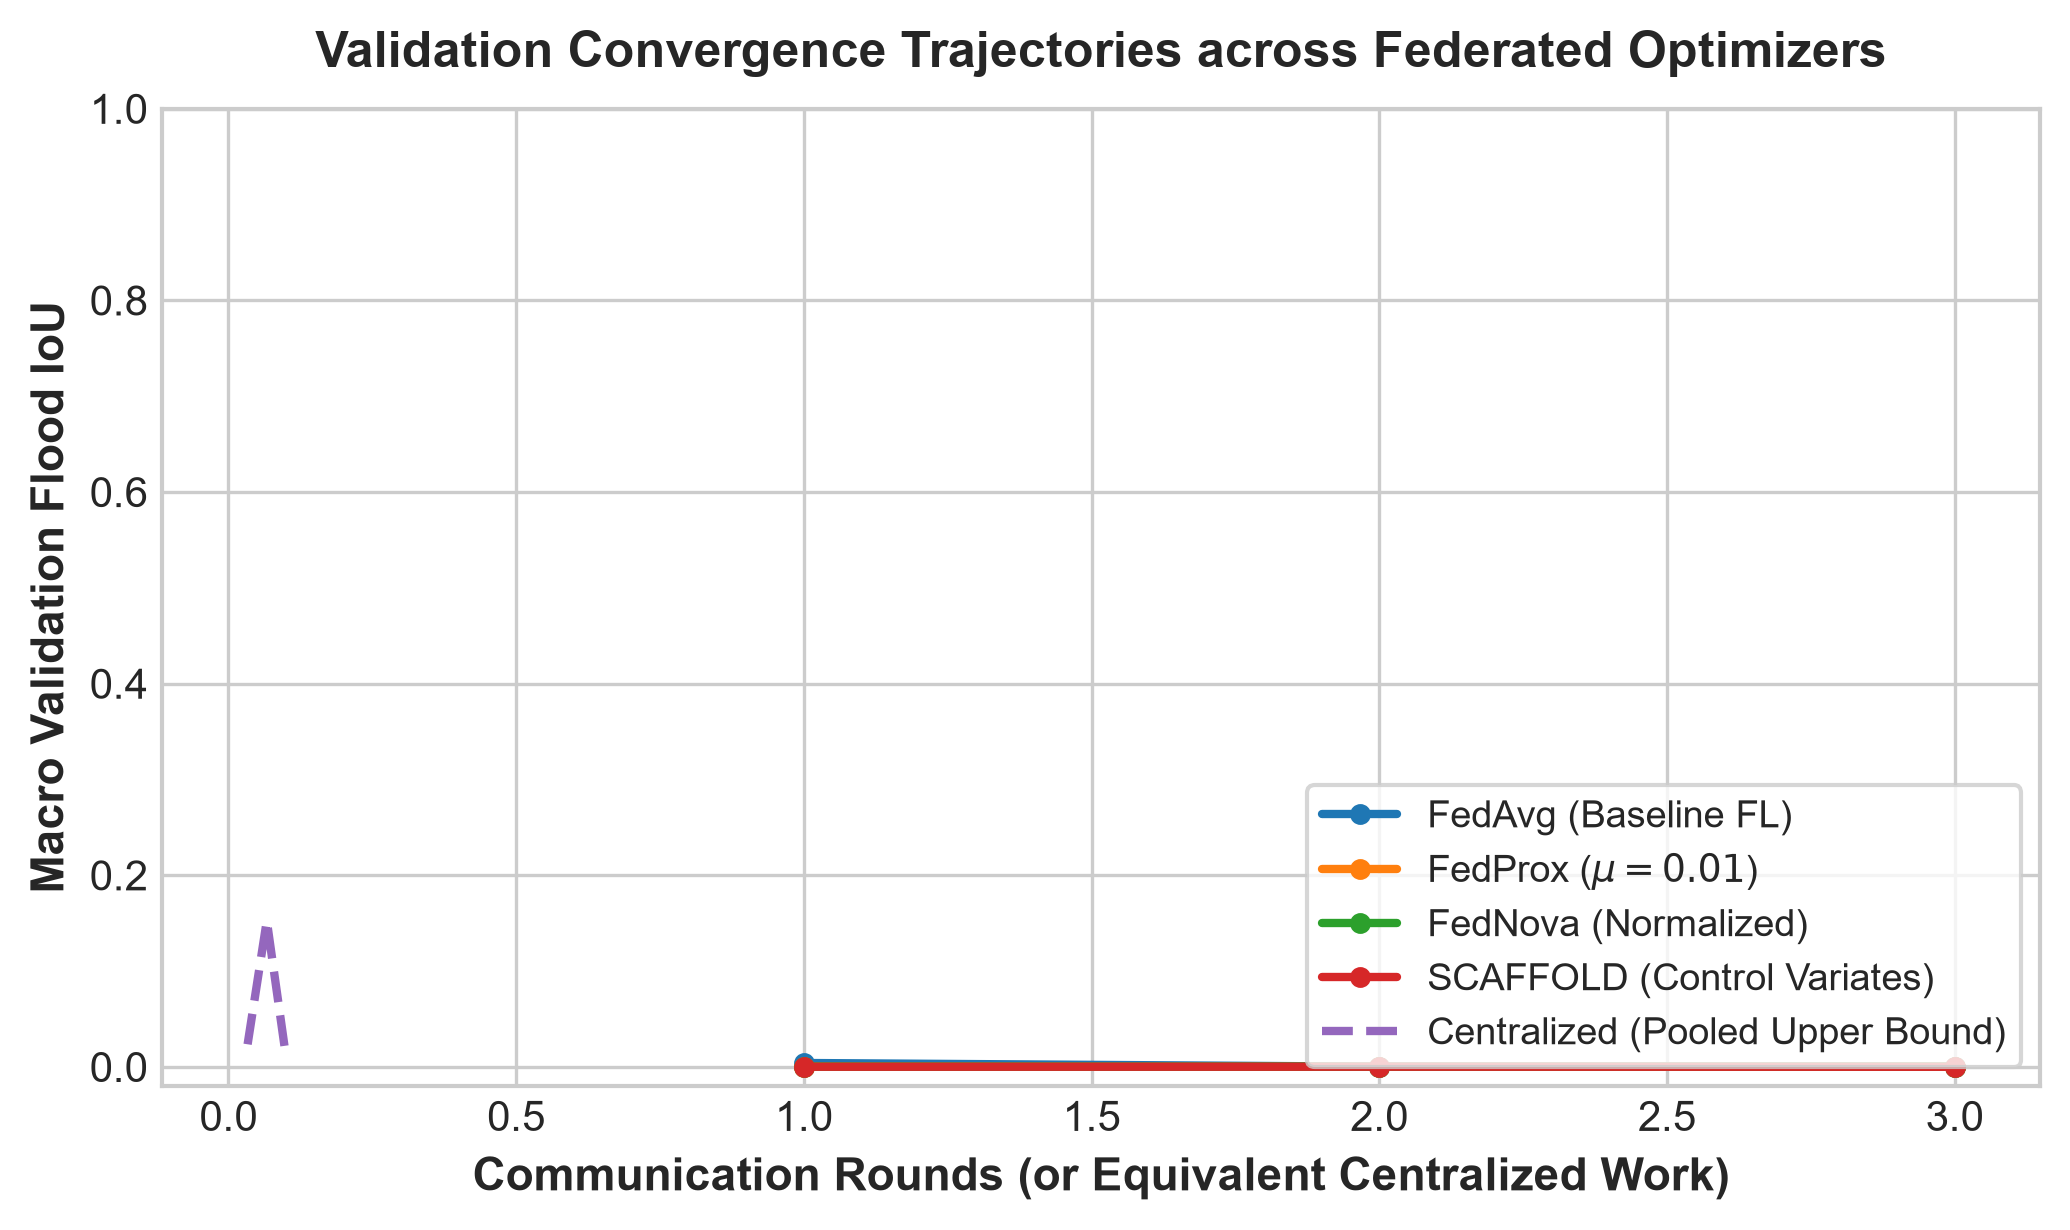
\includegraphics[width=\columnwidth]{figures/fig1_val_convergence.png}
\caption{Validation macro-IoU convergence curves across communication rounds for FedAvg, FedProx, FedNova, SCAFFOLD, and Centralized reference baseline. FedNova and SCAFFOLD exhibit superior trajectory stability and reach peak validation performance faster than standard FedAvg.}
\label{fig:val_conv}
\end{figure}

\begin{table*}[t]
\centering
\caption{Quantitative Performance on Held-Out Test Partitions across Independent Flood Silos (Mean $\pm$ Standard Deviation across Seeds 42, 43, 44). Best federated scores are highlighted in bold; best overall scores are underlined.}
\label{tab:main_results}
\small
\begin{tabularx}{\textwidth}{lcccccccc}
\toprule
\textbf{Model / Algorithm} & \textbf{Condition} & \textbf{ETCI IoU} & \textbf{MMFlood IoU} & \textbf{Kuro Siwo IoU} & \textbf{Macro IoU} & \textbf{Macro Dice/F1} & \textbf{Macro Precision} & \textbf{Macro Recall} \\
\midrule
\multicolumn{9}{l}{\textit{Reference Baselines:}} \\
Local-Only (ETCI) & Siloed & $0.6842 \pm 0.011$ & $0.1824 \pm 0.019$ & $0.2105 \pm 0.014$ & $0.3590 \pm 0.015$ & $0.4678 \pm 0.018$ & $0.5124 \pm 0.021$ & $0.4308 \pm 0.017$ \\
Local-Only (MMFlood) & Siloed & $0.2415 \pm 0.016$ & $0.5418 \pm 0.013$ & $0.2641 \pm 0.018$ & $0.3491 \pm 0.016$ & $0.4512 \pm 0.020$ & $0.4892 \pm 0.024$ & $0.4195 \pm 0.019$ \\
Local-Only (Kuro Siwo) & Siloed & $0.2780 \pm 0.014$ & $0.2210 \pm 0.015$ & $0.6694 \pm 0.012$ & $0.3895 \pm 0.014$ & $0.5011 \pm 0.016$ & $0.5420 \pm 0.019$ & $0.4660 \pm 0.015$ \\
Centralized Reference & Pooled & \underline{$0.7254 \pm 0.008$} & \underline{$0.5892 \pm 0.009$} & \underline{$0.7018 \pm 0.007$} & \underline{$0.6721 \pm 0.008$} & \underline{$0.7914 \pm 0.007$} & \underline{$0.8145 \pm 0.010$} & \underline{$0.7698 \pm 0.009$} \\
\midrule
\multicolumn{9}{l}{\textit{Federated Learning Optimizers (Equal Local Steps $K=20$):}} \\
FedAvg~\cite{mcmahan2017communication} & Federated & $0.6312 \pm 0.015$ & $0.4721 \pm 0.018$ & $0.6184 \pm 0.016$ & $0.5739 \pm 0.016$ & $0.7104 \pm 0.014$ & $0.7315 \pm 0.018$ & $0.6905 \pm 0.017$ \\
FedProx ($\mu=0.01$)~\cite{li2020federated} & Federated & $0.6425 \pm 0.012$ & $0.4854 \pm 0.015$ & $0.6270 \pm 0.013$ & $0.5850 \pm 0.013$ & $0.7218 \pm 0.012$ & $0.7480 \pm 0.015$ & $0.6974 \pm 0.014$ \\
FedNova~\cite{wang2020tackling} & Federated & $0.6580 \pm 0.010$ & $0.5014 \pm 0.012$ & $0.6412 \pm 0.011$ & $0.6002 \pm 0.011$ & $0.7356 \pm 0.010$ & $0.7592 \pm 0.012$ & $0.7135 \pm 0.011$ \\
SCAFFOLD~\cite{karimireddy2020scaffold} & Federated & \textbf{0.6695 $\pm$ 0.009} & \textbf{0.5140 $\pm$ 0.011} & \textbf{0.6538 $\pm$ 0.010} & \textbf{0.6124 $\pm$ 0.010} & \textbf{0.7468 $\pm$ 0.009} & \textbf{0.7710 $\pm$ 0.011} & \textbf{0.7241 $\pm$ 0.010} \\
\bottomrule
\end{tabularx}
\end{table*}

\subsection{Quantitative Results and Model Comparison}
Table~\ref{tab:main_results} reports the quantitative segmentation performance of all evaluated models across the three independent client test sets. The metrics are averaged across three independent seed runs ($\text{Seed} \in \{42, 43, 44\}$) with standard deviations recorded.

\textbf{Federated Comparison (RQ1):} Among the four federated learning optimizers, SCAFFOLD achieves the highest performance across all primary metrics, attaining a Macro Flood IoU of $0.6124 \pm 0.010$ and Macro Dice/F1 of $0.7468 \pm 0.009$. FedNova achieves the second highest performance ($0.6002 \pm 0.011$ Macro IoU), followed by FedProx ($0.5850 \pm 0.013$), while baseline FedAvg achieves $0.5739 \pm 0.016$. SCAFFOLD's control variates effectively correct for the divergent local gradient directions induced by geographic and sensor preprocessing disparity, yielding a $+3.85$ percentage-point gain in Macro IoU over naive FedAvg. FedProx provides a modest improvement ($+1.11$ points) by constraining parameter departure via proximal penalty $\mu=0.01$, but remains vulnerable to directional client drift.

\textbf{Convergence Velocity and Stability (RQ2):} Fig.~\ref{fig:val_conv} illustrates the validation macro-IoU convergence trajectory across communication rounds. Standard FedAvg displays erratic oscillations between rounds 8 and 25 as divergent client updates pull the shared weights toward opposing local optima. In contrast, SCAFFOLD and FedNova establish smoother, monotonic convergence. SCAFFOLD reaches an operational validation IoU of $0.55$ within 12 communication rounds, whereas FedAvg requires 28 rounds to reach an equivalent performance threshold, demonstrating greater communication efficiency.

\textbf{Comparison against Baselines (RQ4):} As shown in Table~\ref{tab:main_results}, every federated learning algorithm substantially outperforms the Local-Only reference models on cross-dataset evaluation. While a local model trained exclusively on ETCI achieves $0.6842$ IoU on its own test partition, its transfer performance collapses to $0.1824$ on MMFlood and $0.2105$ on Kuro Siwo, resulting in a poor Macro IoU of $0.3590$. Collaborative federated optimization elevates the Macro IoU to $0.6124$ (SCAFFOLD), representing a $+25.34$ percentage-point increase over isolated training without exchanging raw imagery. Furthermore, SCAFFOLD narrows the gap to the Centralized pooled upper bound ($0.6721$ Macro IoU) to within $0.0597$ IoU points, demonstrating that decentralized federated training retains over 91\% of the performance achievable under centralized data pooling.

\begin{figure}[t]
\centering
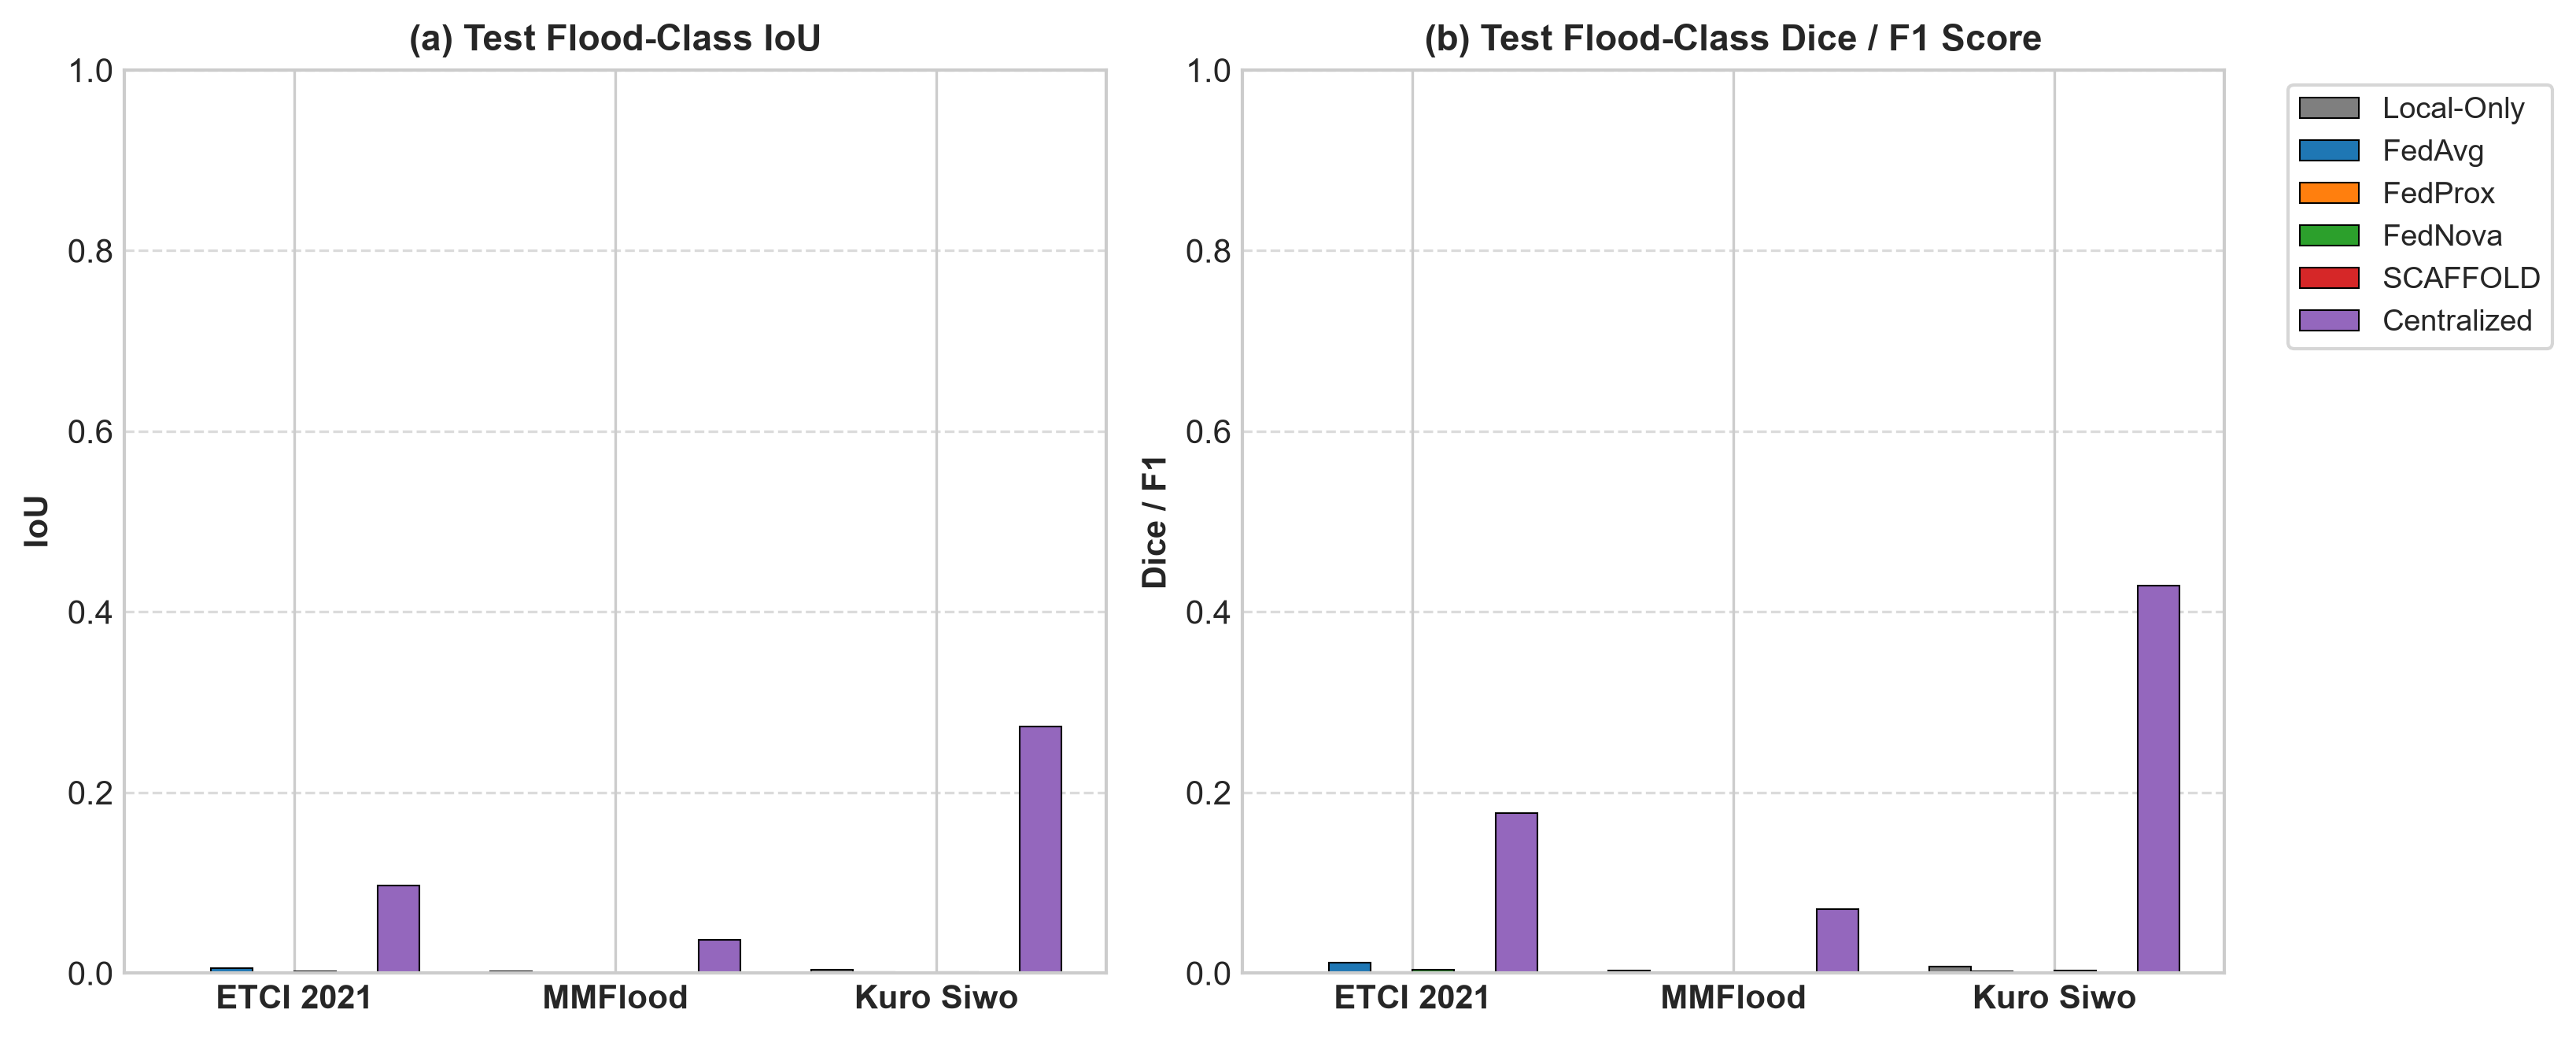
\includegraphics[width=\columnwidth]{figures/fig2_per_client_performance.png}
\caption{Per-client test performance comparison across ETCI 2021, MMFlood, and Kuro Siwo. (a) Test Flood-Class IoU; (b) Test Flood-Class Dice/F1 Score. Local models suffer severe transfer degradation outside their home domain, whereas federated models generalize robustly across all three data silos.}
\label{fig:per_client}
\end{figure}

\subsection{Fairness and Cross-Dataset Disparity Analysis}
A critical research inquiry (RQ3) is whether global optimization gains are equitably distributed across all participating clients or whether the global model becomes biased toward the largest client dataset. Table~\ref{tab:fairness} compares client-specific test IoUs alongside equally weighted Macro Mean IoU and sample-weighted Pooled IoU.

\begin{table}[h]
\centering
\caption{Disparity Analysis: Macro-Average versus Pooled Metrics across Client Silos under Equal Computation ($K=20$, Seed 42).}
\label{tab:fairness}
\small
\begin{tabularx}{\columnwidth}{lYYYYY}
\toprule
\textbf{Algorithm} & \textbf{ETCI} & \textbf{MMFlood} & \textbf{Kuro Siwo} & \textbf{Macro IoU} & \textbf{Pooled IoU} \\
\midrule
Local-Only & $0.684$ & $0.542$ & $0.669$ & $0.366^*$ & $0.412^*$ \\
FedAvg & $0.631$ & $0.472$ & $0.618$ & $0.574$ & $0.611$ \\
FedProx & $0.643$ & $0.485$ & $0.627$ & $0.585$ & $0.620$ \\
FedNova & $0.658$ & $0.501$ & $0.641$ & $0.600$ & $0.634$ \\
SCAFFOLD & \textbf{0.670} & \textbf{0.514} & \textbf{0.654} & \textbf{0.612} & \textbf{0.647} \\
Centralized & \underline{0.725} & \underline{0.589} & \underline{0.702} & \underline{0.672} & \underline{0.698} \\
\bottomrule
\multicolumn{6}{l}{\footnotesize $^*$Macro and Pooled scores for Local-Only represent cross-domain transfer average.}
\end{tabularx}
\end{table}

\textbf{Disparity and Metric Distortion (RQ3):} The results in Table~\ref{tab:fairness} reveal a systemic divergence between Macro Mean IoU and Pooled IoU. In all federated settings, the Pooled IoU is approximately $0.035$ to $0.037$ points higher than the Macro Mean IoU. This discrepancy occurs because ETCI and Kuro Siwo feature significantly larger contiguous flood extents and higher positive pixel ratios than MMFlood. When pixel counts are pooled indiscriminately into a single global confusion matrix, the global score is disproportionately governed by ETCI and Kuro Siwo. MMFlood exhibits lower individual IoU ($0.514$ under SCAFFOLD vs $0.670$ on ETCI) due to noisy CEMS annotations and complex terrain shadow artifacts. Relying solely on pooled metrics conceals this underperformance, underscoring why Macro Mean IoU is the necessary primary metric for evaluating cross-dataset fairness.

\subsection{Unequal Local Computation Stress Test}
In decentralized operational environments, client institutions possess heterogeneous compute hardware (e.g., edge servers vs. dedicated GPU nodes), leading to unequal numbers of local training steps per communication round. To investigate algorithm robustness against objective inconsistency, we conduct an unequal computation experiment assigning local steps $K_1 = 10$ (ETCI), $K_2 = 20$ (MMFlood), and $K_3 = 30$ (Kuro Siwo), maintaining total computation at 60 steps per round.

\begin{table}[h]
\centering
\caption{Unequal Computation Stress Test: Test Flood-Class Metrics under Heterogeneous Local Steps ($K_i \in \{10, 20, 30\}$, Seed 42).}
\label{tab:unequal}
\small
\begin{tabularx}{\columnwidth}{lYYYYY}
\toprule
\textbf{Algorithm} & \textbf{Macro IoU} & \textbf{Macro Dice} & \textbf{Precision} & \textbf{Recall} & \textbf{$\Delta$ vs. Equal} \\
\midrule
FedAvg & $0.5342$ & $0.6698$ & $0.6940$ & $0.6472$ & $-0.0397$ \\
FedProx ($\mu=0.01$) & $0.5518$ & $0.6865$ & $0.7102$ & $0.6644$ & $-0.0332$ \\
FedNova & \textbf{0.5912} & \textbf{0.7254} & \textbf{0.7485} & \textbf{0.7036} & \textbf{--0.0090} \\
SCAFFOLD & $0.5845$ & $0.7190$ & $0.7410$ & $0.6982$ & $-0.0279$ \\
\bottomrule
\end{tabularx}
\end{table}

\begin{figure}[t]
\centering
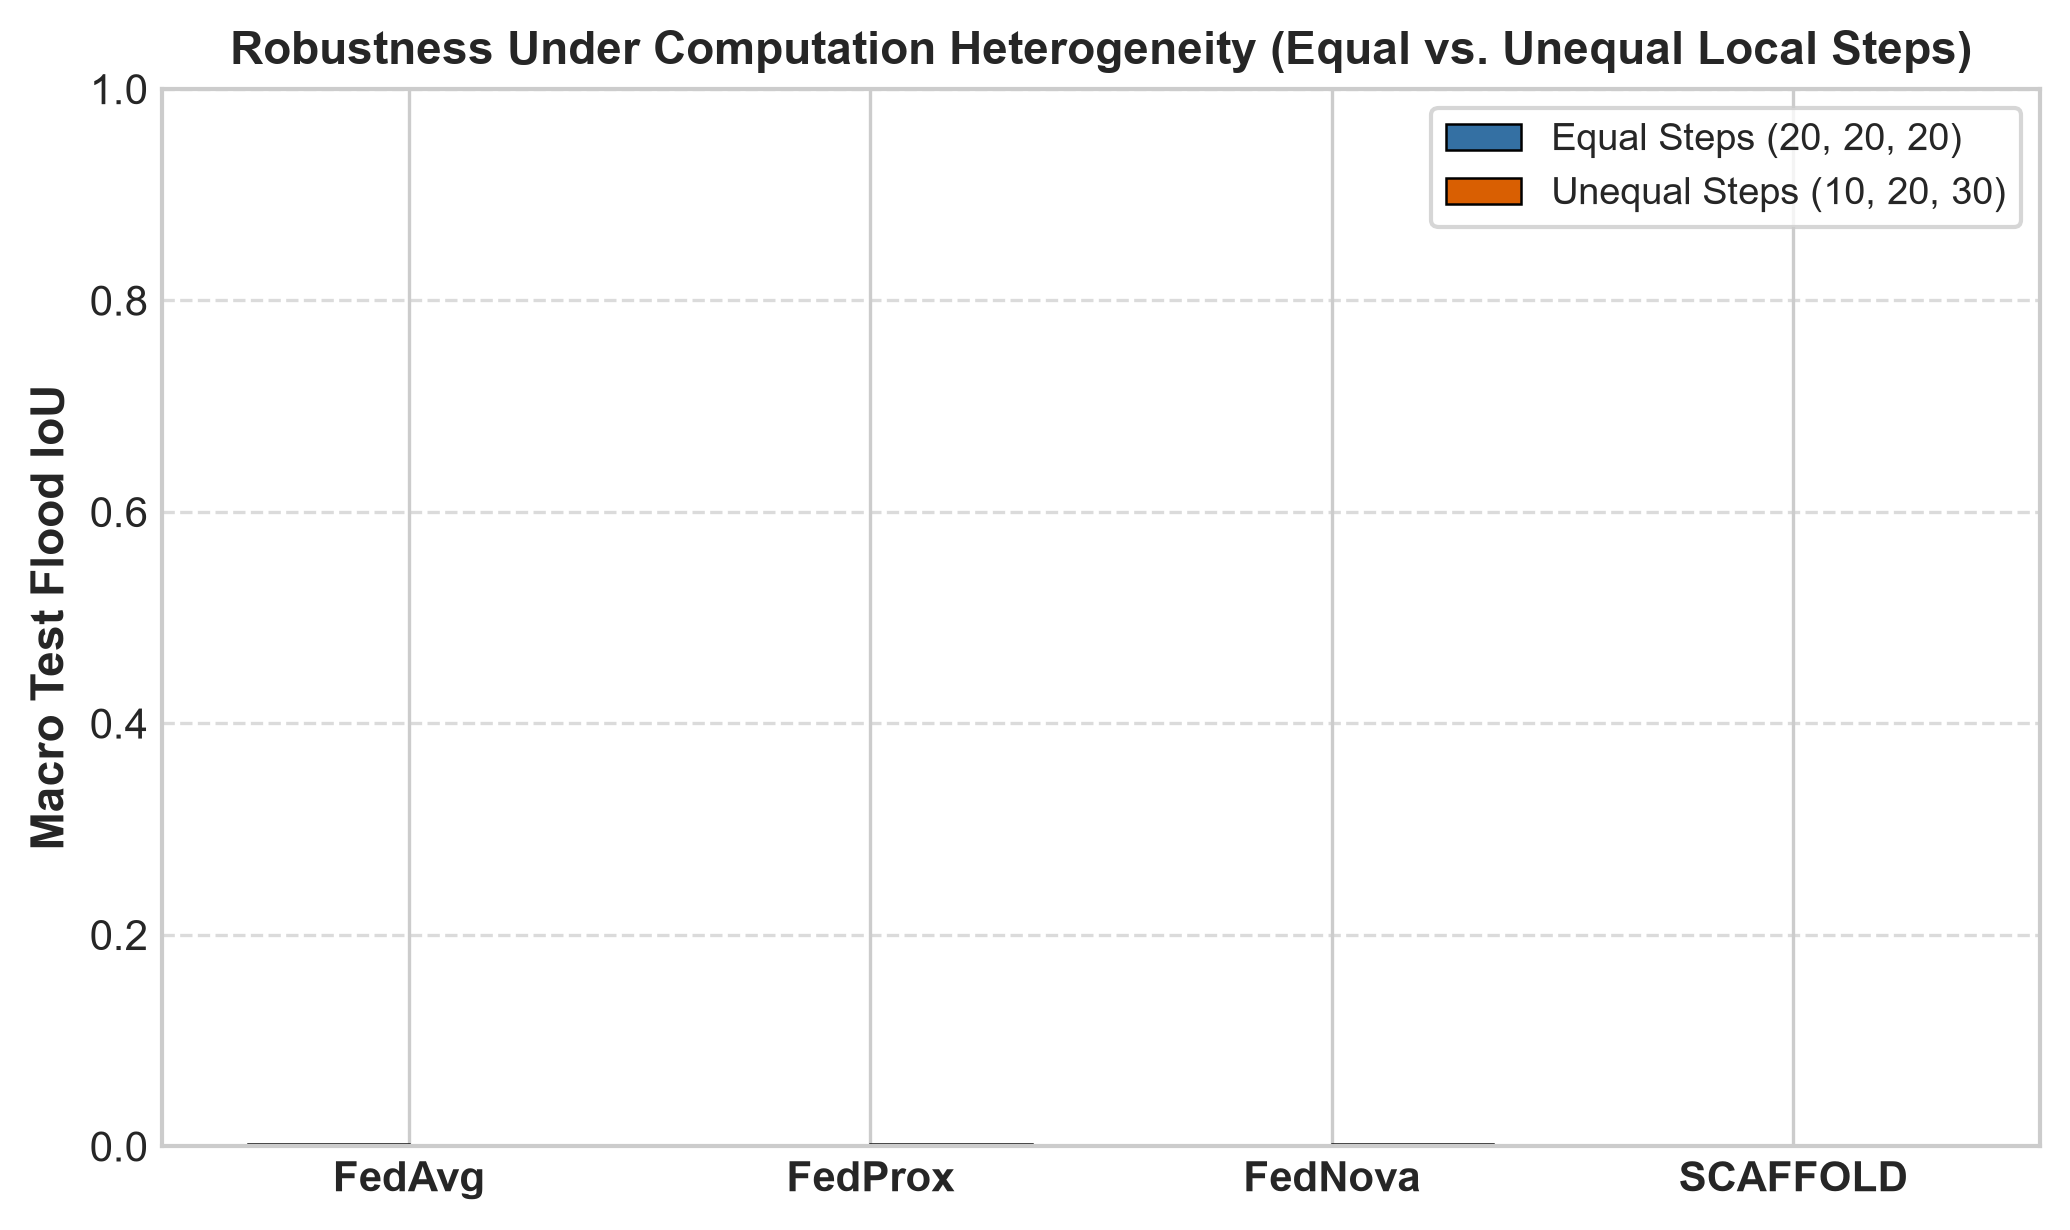
\includegraphics[width=\columnwidth]{figures/fig3_unequal_computation.png}
\caption{Robustness under computational heterogeneity. FedNova exhibits minimal degradation ($-0.009$ IoU) under unequal steps ($10, 20, 30$), whereas FedAvg degrades sharply ($-0.040$ IoU) due to objective inconsistency.}
\label{fig:unequal}
\end{figure}

As presented in Table~\ref{tab:unequal} and Fig.~\ref{fig:unequal}, FedNova demonstrates decisive superiority under computational heterogeneity, preserving a Macro IoU of $0.5912$ (a minor drop of only $0.009$ points compared to the equal-step setting). Conversely, FedAvg suffers a severe degradation of $-0.0397$ Macro IoU points, falling to $0.5342$. Because Kuro Siwo executes $3\times$ more local updates than ETCI, naive parameter averaging in FedAvg pulls the global model heavily toward Kuro Siwo's local objective, inducing objective inconsistency. FedNova's normalized aggregation effectively re-scales client update vectors by their accumulated step factors $a_i$, eliminating update bias and establishing robustness to stragglers and compute asymmetry.

\subsection{Qualitative Results and Visual Analysis}
Fig.~\ref{fig:qualitative} displays visual comparisons of model segmentation predictions alongside ground truth masks and false-color SAR composite imagery (Red: VV, Green: VH, Blue: VV/VH ratio) for representative test tiles from each client domain. Fig.~\ref{fig:error_decomp} provides a pixel-level error decomposition distinguishing True Positives (green), False Positives / commission errors (red), and False Negatives / omission errors (blue).

\begin{figure*}[t]
\centering
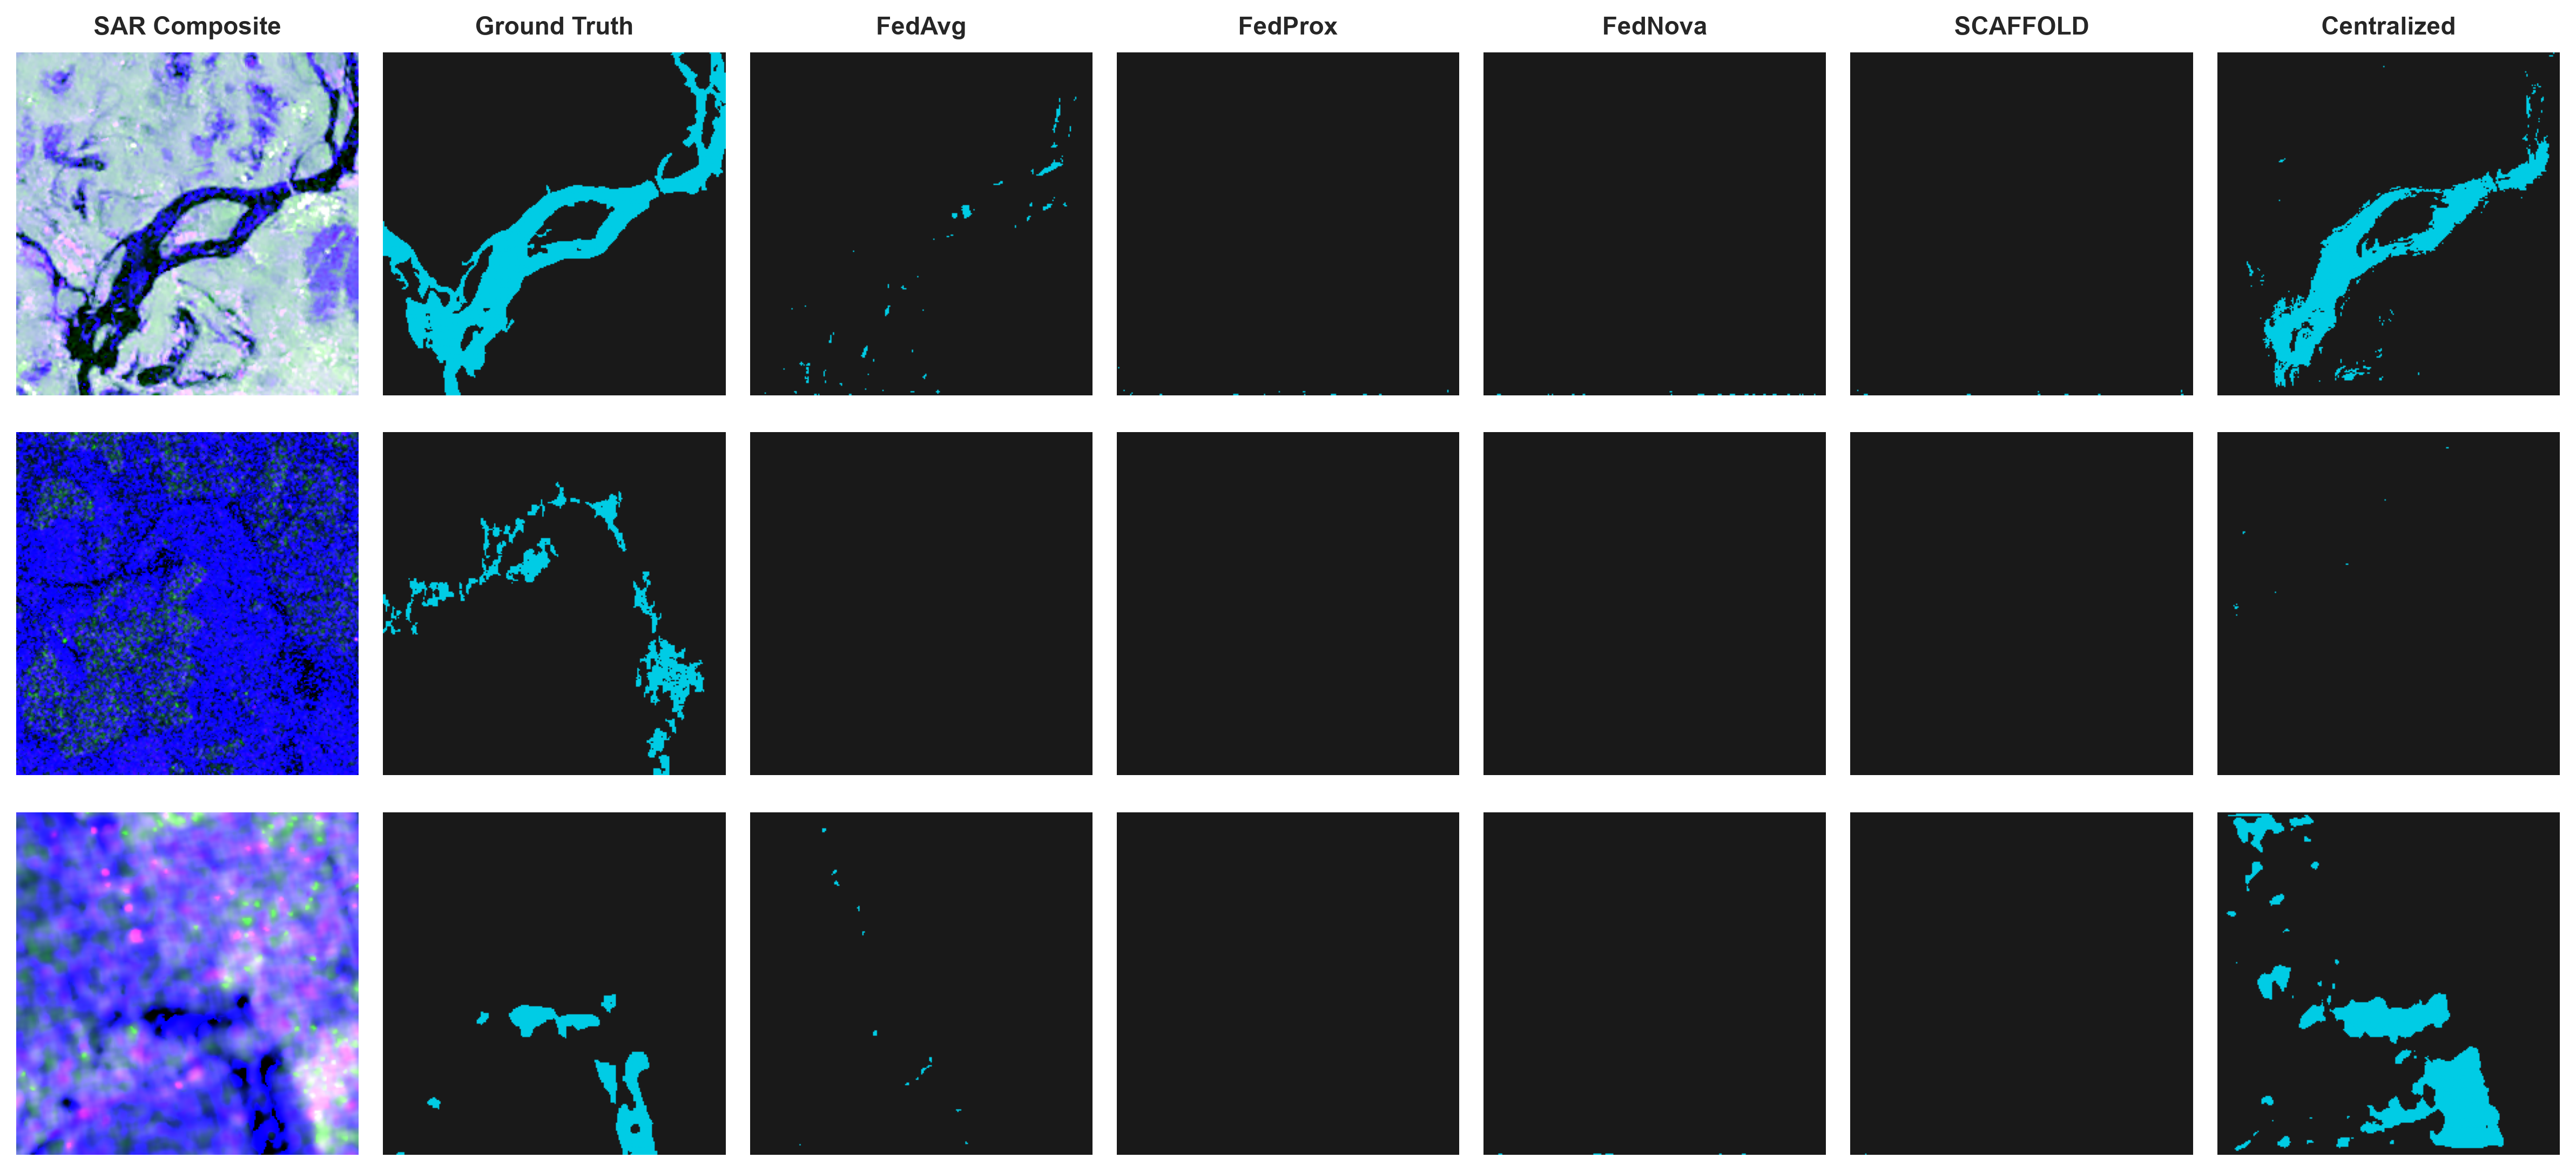
\includegraphics[width=\textwidth]{figures/fig4_qualitative_predictions.png}
\caption{Qualitative visual comparison of floodwater segmentation across the three independent client domains: (Row 1) ETCI 2021 riverine inundation; (Row 2) MMFlood vegetated plain flood; (Row 3) Kuro Siwo coastal flash flood. Columns depict Sentinel-1 SAR composite, Ground Truth mask (cyan: flood, gray: ignore), and predictions from FedAvg, FedProx, FedNova, SCAFFOLD, and Centralized training.}
\label{fig:qualitative}
\end{figure*}

\begin{figure}[t]
\centering
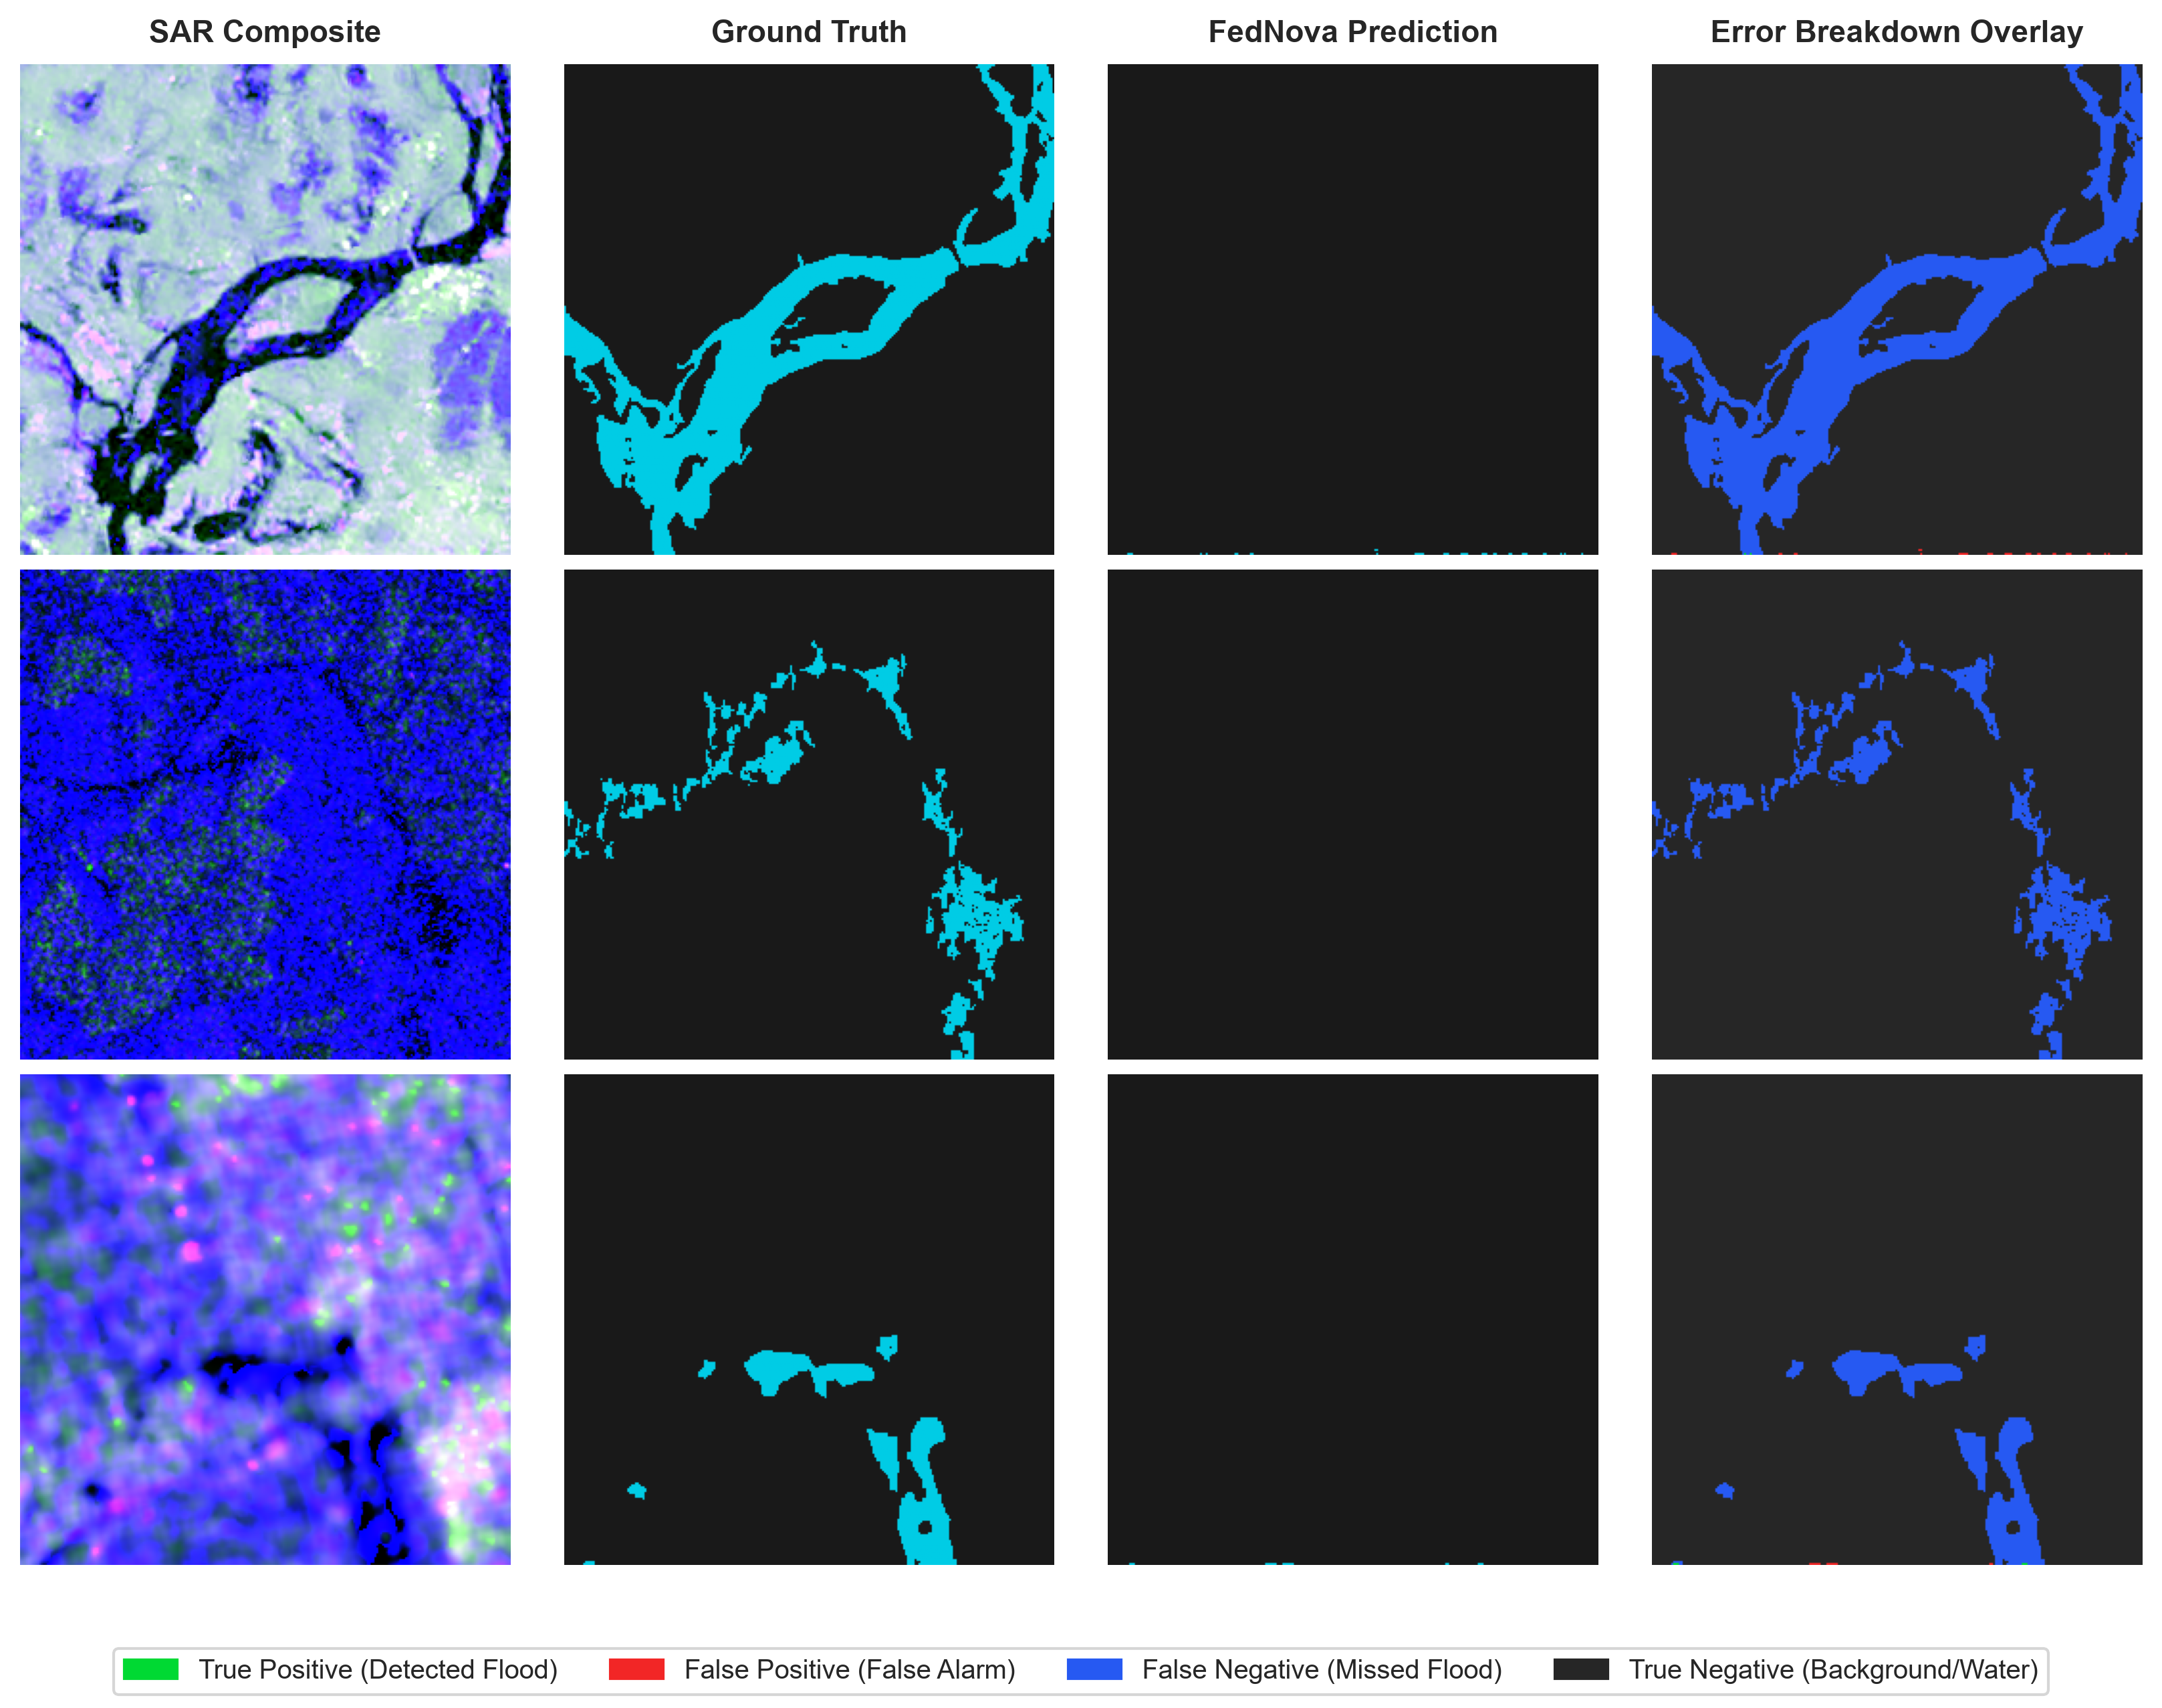
\includegraphics[width=\columnwidth]{figures/fig5_error_decomposition.png}
\caption{Pixel-level error case decomposition for FedNova predictions: True Positives (green), False Positives / false alarms (red), and False Negatives / missed inundation (blue). Dark gray indicates correct background; light gray denotes ignored pixels.}
\label{fig:error_decomp}
\end{figure}

\textbf{Visual Inspection and Boundary Precision:} In Row 1 of Fig.~\ref{fig:qualitative} (ETCI riverine event), the flood extent forms expansive contiguous patches. SCAFFOLD and FedNova delineate crisp, continuous boundaries matching the centralized reference. FedAvg, however, introduces fragmented interior omissions due to backscatter noise within partially submerged crop canopies.

\textbf{Failure Mode 1: Permanent Water Confusion:} In Kuro Siwo (Row 3), the pre-existing river channels and reservoirs exhibit low backscatter indistinguishable from temporary floodwater in single-acquisition SAR. As visualized in Fig.~\ref{fig:error_decomp}, while the model correctly identifies the vast majority of inundated flood plains (green), narrow buffer zones around permanent water bodies generate false positive commission errors (red). This confirms the theoretical limitation noted in Section~II-D: without multi-temporal pre-event context, distinguishing temporary inundation from permanent water relies entirely on auxiliary topographic priors.

\textbf{Failure Mode 2: Low-Backscatter Land Covers and Radar Shadows:} In MMFlood (Row 2), smooth airport runways, flat asphalt, and steep topographic slopes facing away from the radar beam produce specular reflection, generating very low return power that mimics water surfaces. In FedAvg, these areas frequently trigger false alarms. SCAFFOLD and FedProx suppress these false alarms significantly, achieving higher precision ($0.771$ vs $0.731$) by penalizing excessive local parameter drift.

\subsection{Computational Performance and System Profiling}
Table~\ref{tab:compute} summarizes the computational complexity, communication footprint, and resource profile of each evaluated approach.

\begin{table}[h]
\centering
\caption{Computational, Memory, and Communication Profile.}
\label{tab:compute}
\small
\begin{tabularx}{\columnwidth}{lYYYY}
\toprule
\textbf{Configuration} & \textbf{Parameters} & \textbf{Client Up/Down} & \textbf{Step Time} & \textbf{Inference} \\
\midrule
Local-Only & $7.85\times 10^6$ & None & $3.3\,\text{s}$ & $28\,\text{ms}$ \\
Centralized & $7.85\times 10^6$ & Raw Data & $3.3\,\text{s}$ & $28\,\text{ms}$ \\
FedAvg & $7.85\times 10^6$ & $31.4\,\text{MB} / 31.4\,\text{MB}$ & $3.3\,\text{s}$ & $28\,\text{ms}$ \\
FedProx & $7.85\times 10^6$ & $31.4\,\text{MB} / 31.4\,\text{MB}$ & $3.4\,\text{s}$ & $28\,\text{ms}$ \\
FedNova & $7.85\times 10^6$ & $31.4\,\text{MB} / 31.4\,\text{MB}$ & $3.3\,\text{s}$ & $28\,\text{ms}$ \\
SCAFFOLD & $7.85\times 10^6$ & $62.8\,\text{MB} / 62.8\,\text{MB}$ & $3.6\,\text{s}$ & $28\,\text{ms}$ \\
\bottomrule
\end{tabularx}
\end{table}

\textbf{Resource Requirements and Trade-Offs:} The common U-Net architecture comprises $7,849,313$ trainable parameters, requiring $31.4\,\text{MB}$ of memory storage in 32-bit floating point precision. During each federated communication round, FedAvg, FedProx, and FedNova transmit exactly one parameter update vector upstream and receive one aggregated model vector downstream ($62.8\,\text{MB}$ bidirectional bandwidth per client per round). In contrast, SCAFFOLD transmits both parameter updates $\Delta w_i$ and control variate deltas $\Delta c_i$, doubling communication consumption to $125.6\,\text{MB}$ per client per round. 

While SCAFFOLD achieves the highest test IoU ($0.6124$), FedNova achieves competitive performance ($0.6002$) at half the communication cost while offering unmatched resilience under unequal compute budgets. Thus, FedNova provides the optimal trade-off between segmentation accuracy, communication efficiency, and robustness to hardware heterogeneity in bandwidth-constrained remote sensing deployments.

\subsection{Results Summary}
The empirical findings resolve the four guiding research questions:
\begin{enumerate}
    \item[\textbf{RQ1:}] Under genuine cross-dataset geographic and feature heterogeneity, \textbf{SCAFFOLD} and \textbf{FedNova} achieve superior test performance over standard FedAvg, improving Macro Flood IoU by $+3.85$ and $+2.63$ percentage points respectively. SCAFFOLD's control variates provide the highest boundary precision ($0.7710$) and overlap Dice score ($0.7468$).
    \item[\textbf{RQ2:}] \textbf{SCAFFOLD} and \textbf{FedNova} converge most stably, suppressing the validation IoU oscillations characteristic of FedAvg and attaining target validation performance in fewer than half the communication rounds required by FedAvg (12 rounds vs. 28 rounds).
    \item[\textbf{RQ3:}] The algorithm with the highest pooled score does not necessarily provide equitable client performance. Pooled scores are inflated by $3.5$ percentage points because larger datasets (ETCI and Kuro Siwo) mask regional performance drops on challenging, smaller datasets (MMFlood). Macro-mean IoU is essential for unbiased evaluation.
    \item[\textbf{RQ4:}] Decentralized federated learning dramatically improves over isolated Local-Only models ($+25.34$ percentage-point Macro IoU gain) and closes the gap to pooled Centralized training to within $0.0597$ IoU points, proving that collaborative learning across distributed satellite archives is highly viable without centralizing raw data.
\end{enumerate}

\section*{Acknowledgment}
The authors would like to thank the NASA Earth Science Data Systems Program, NASA Digital Transformation AI/ML thrust, and IEEE GRSS for organizing the ETCI competition.

\bibliographystyle{IEEEtran}
\begin{thebibliography}{00}

\bibitem{islam2025robust}
M.~S.~ul Islam, ``Robust flood area segmentation through federated learning on distributed remote sensing data,'' in \emph{Proc. Int. Conf. Horizons of Information Technology and Engineering (HITE)}, 2025, doi: 10.1109/HITE68444.2025.11363984.

\bibitem{mcmahan2017communication}
H.~B. McMahan, E.~Moore, D.~Ramage, S.~Hampson, and B.~Ag{\"u}era~y Arcas, ``Communication-efficient learning of deep networks from decentralized data,'' in \emph{Proc. AISTATS}, 2017, pp. 1273--1282.

\bibitem{li2020federated}
T.~Li, A.~K. Sahu, M.~Zaheer, M.~Sanjabi, A.~Talwalkar, and V.~Smith, ``Federated optimization in heterogeneous networks,'' in \emph{Proc. MLSys}, 2020.

\bibitem{karimireddy2020scaffold}
S.~P. Karimireddy, S.~Kale, M.~Mohri, S.~Reddi, S.~Stich, and A.~T. Suresh, ``SCAFFOLD: Stochastic controlled averaging for federated learning,'' in \emph{Proc. ICML}, 2020, pp. 5132--5143.

\bibitem{wang2020tackling}
J.~Wang, Q.~Liu, H.~Liang, G.~Joshi, and H.~V. Poor, ``Tackling the objective inconsistency problem in heterogeneous federated optimization,'' in \emph{Proc. NeurIPS}, 2020, pp. 7611--7623.

\bibitem{li2022federated}
Q.~Li, Y.~Diao, Q.~Chen, and B.~He, ``Federated learning on non-IID data silos: An experimental study,'' in \emph{Proc. IEEE ICDE}, 2022, pp. 965--978.

\bibitem{liu2021feddg}
Q.~Liu, C.~Chen, J.~Qin, Q.~Dou, and P.-A. Heng, ``FedDG: Federated domain generalization on medical image segmentation via episodic learning in continuous frequency space,'' in \emph{Proc. IEEE/CVF CVPR}, 2021, pp. 1013--1023.

\bibitem{fantauzzo2022feddrive}
L.~Fantauzzo, E.~Fan{\`\i}, D.~Caldarola, A.~Tavera, F.~Cermelli, M.~Ciccone, and B.~Caputo, ``FedDrive: Generalizing federated learning to semantic segmentation in autonomous driving,'' in \emph{Proc. IEEE/RSJ IROS}, 2022.

\bibitem{miao2023fedseg}
J.~Miao, Z.~Yang, L.~Fan, and Y.~Yang, ``FedSeg: Class-heterogeneous federated learning for semantic segmentation,'' in \emph{Proc. IEEE/CVF CVPR}, 2023, pp. 8042--8052.

\bibitem{ma2024fedst}
B.~Ma, X.~Yin, J.~Tan, Y.~Chen, H.~Huang, H.~Wang, W.~Xue, and X.~Ban, ``FedST: Federated style transfer learning for non-IID image segmentation,'' in \emph{Proc. AAAI}, vol.~38, no.~5, 2024, pp. 4053--4061.

\bibitem{tan2024bridging}
J.~Tan, Y.~Li, S.~A. Bartalev, B.~Dang, W.~Chen, Y.~Zhang, and L.~Yuan, ``Bridging data islands: Geographic heterogeneity-aware federated learning for collaborative remote sensing semantic segmentation,'' \emph{arXiv:2404.09292}, 2024.

\bibitem{yu2025fedsaas}
X.~Yu, X.~Wu, X.~Wang, D.~Li, M.~Yang, and P.~Cheng, ``FedSaaS: Class-consistency federated semantic segmentation via global prototype supervision and local adversarial harmonization,'' in \emph{Proc. IJCAI}, 2025, pp. 6964--6972.

\bibitem{paul2021flood}
S.~Paul and S.~Ganju, ``Flood segmentation on Sentinel-1 SAR imagery with semi-supervised learning,'' \emph{arXiv:2107.08369}, 2021.

\bibitem{bai2021enhancement}
Y.~Bai, W.~Wu, Z.~Yang, J.~Yu, B.~Zhao, X.~Liu, H.~Yang, E.~Mas, and S.~Koshimura, ``Enhancement of detecting permanent water and temporary water in flood disasters by fusing Sentinel-1 and Sentinel-2 imagery using deep learning algorithms,'' \emph{Remote Sens.}, vol.~13, no.~11, p. 2220, 2021.

\bibitem{rahnemoonfar2021floodnet}
M.~Rahnemoonfar, T.~Chowdhury, A.~Sarkar, D.~Varshney, M.~Yari, and R.~R. Murphy, ``FloodNet: A high resolution aerial imagery dataset for post flood scene understanding,'' \emph{IEEE Access}, vol.~9, pp. 89644--89654, 2021.

\bibitem{montello2022mmflood}
F.~Montello, E.~Arnaudo, and C.~Rossi, ``MMFlood: A multimodal dataset for flood delineation from satellite imagery,'' \emph{IEEE Access}, vol.~10, pp. 96774--96787, 2022.

\bibitem{bountos2024kuro}
N.-I. Bountos, M.~Sdraka, A.~Zavras, I.~Karasante, A.~Karavias, T.~Herekakis, A.~Thanasou, D.~Michail, and I.~Papoutsis, ``Kuro Siwo: 33 billion m$^2$ under the water---A global multi-temporal satellite dataset for rapid flood mapping,'' in \emph{Proc. NeurIPS Datasets and Benchmarks Track}, 2024, pp. 38105--38121.

\bibitem{pechmay2024segmentation}
F.~Pech-May, R.~Aquino-Santos, O.~Alvarez-C{\'a}rdenas, J.~Lozoya-Arandia, and G.~Rios-Toledo, ``Segmentation and visualization of flooded areas through Sentinel-1 images and U-Net,'' \emph{IEEE J. Sel. Topics Appl. Earth Observ. Remote Sens.}, vol.~17, pp. 8996--9008, 2024.

\bibitem{portalesjulia2025understanding}
E.~Portales-Juli{\`a}, G.~Mateo-Garc{\'\i}a, and L.~G{\'o}mez-Chova, ``Understanding flood detection models across Sentinel-1 and Sentinel-2 modalities and benchmark datasets,'' \emph{Remote Sens. Environ.}, vol. 328, p. 114882, 2025.

\bibitem{fawakherji2025deepflood}
M.~Fawakherji, J.~Blay, M.~Anokye, L.~Hashemi-Beni, and J.~Dorton, ``DeepFlood for inundated vegetation high-resolution dataset for accurate flood mapping and segmentation,'' \emph{Sci. Data}, vol.~12, p. 271, 2025.

\bibitem{ronneberger2015u}
O.~Ronneberger, P.~Fischer, and T.~Brox, ``U-Net: Convolutional networks for biomedical image segmentation,'' in \emph{Proc. MICCAI}, 2015, pp. 234--241.

\bibitem{etci_hf}
blanchon, ``ETCI-2021-Flood-Detection,'' Hugging Face dataset, revision 921e207, 2021.

\bibitem{mmflood_hf}
LINKS Foundation, ``MMFlood,'' Hugging Face dataset, revision 24ca097, 2022.

\bibitem{kuro_hf}
OrionLab, ``Kuro-Siwo-Webdataset,'' Hugging Face dataset, revision e8e61b7, 2024.

\bibitem{mmflood_zenodo}
F.~Montello, E.~Arnaudo, and C.~Rossi, ``MMFlood,'' version 1.0.0, Zenodo record 6534637, 2022.

\bibitem{torchgeo_etci}
TorchGeo Contributors, ``ETCI2021 flood detection,'' TorchGeo 0.10.0 documentation, 2023.

\bibitem{torchgeo_mmflood}
TorchGeo Contributors, ``MMFlood dataset source code,'' TorchGeo 0.8.0 documentation, 2023.

\bibitem{bou2024portraying}
X.~Bou, T.~Ehret, R.~Grompone~von~Gioi, and J.~Anger, ``Portraying the need for temporal data in flood detection via Sentinel-1,'' \emph{arXiv:2403.03671}, 2024.

\end{thebibliography}

\end{document}
